% =========================================================================
% Capítulo 2 - Tema 01: Dinámica de la Partícula
% =========================================================================

\section{Ejercicios de Dinámica de la Partícula}

Los siguientes problemas aplican la segunda ley de Newton, el teorema
trabajo-energía y el impulso-momento al análisis de una partícula individual
sometida a restricciones geométricas, resortes y marcos de referencia móviles.

\subsection{Ejercicios}

% =========================================================================
% Capítulo 2: Cinética de la partícula
% Tema 01: Dinámica de la partícula
% Problema 01: Partícula en un disco con rodadura
% =========================================================================
\subsubsection{Partícula en un disco con rodadura}

Un disco sin masa de radio $R$ rueda sin resbalar a una velocidad angular constante $\omega$ a lo largo de una superficie horizontal. Una partícula de masa $m$ se desliza en una ranura cortada a lo largo de una dirección radial del disco, la cual se encuentra llena de un fluido que genera fricción en el movimiento de la partícula, cuyo coeficiente de fricción es $\nu$. Unido a la partícula hay un resorte lineal con constante de resorte $K$, largo natural $r_0$ y punto de unión $O$, donde $O$ está ubicado en el centro del disco.

\begin{enumerate}[label=(\alph*)]
    \item Determine marcos de referencia y defina sistemas de coordenadas.
    \item Realice un análisis cinético de las fuerzas que actúan sobre la partícula. Para esto, haga un diagrama de cuerpo libre de la partícula y especifique las fuerzas actuantes sobre ella.
    \item Determine la ecuación diferencial de movimiento de la partícula en términos de la variable $r$ usando la Segunda Ley de Newton. ($\ddot{r}=f(r,\dot r,t)$)
\end{enumerate}

\begin{figure}[!ht]
    \centering
    \begin{tikzpicture}[>=Latex, scale=1.3]
        
        % --- CONFIGURACIÓN ---
        \def\R{2.0}      % Radio del disco
        \def\ang{40}    % Ángulo omega*t
        \def\distP{1.2} % Distancia r de la partícula
        
        % Suelo (Hachurado)
        \fill[pattern=north east lines] (-3, -\R-0.2) rectangle (3, -\R);
        \draw[thick] (-3, -\R) -- (3, -\R);
        \node[right] at (1.5, -\R+0.3) {Sin dezlizamiento};
        
        % Disco
% Disco con sombreado radial para mayor realismo
        \draw[thick, inner color=gray!5, outer color=gray!30] (0,0) circle (\R);
        
        % Opcional: un borde más marcado
        \draw[thick] (0,0) circle (\R);
        \draw[dashed] (0,0) -- (0, \R+0.5); % Eje vertical de referencia
        
        % Centro O
        \filldraw (0,0) circle (1.5pt) node[left, xshift=-2pt] {$O$};
        
        % Ranura y Partícula
        \begin{scope}[rotate={- \ang}] % Rotación horaria como en el dibujo
            % Ranura (rectángulo estilizado)
            \draw[fill=white] (0.3, -0.15) rectangle (\R-0.2, 0.15);
            
            % Resorte
            \draw[decoration={coil,aspect=0.4, amplitude=3pt, segment length=4pt}, decorate] (0,0) -- (\distP, 0) node[midway,above right] {$K$};
            
            % Partícula
            \filldraw (\distP, 0) circle (2.5pt);
            
            % Etiqueta r
            \draw[<->] (0, -0.4) -- (\distP, -0.4) node[midway, below] {$r$};
        \end{scope}
        
        % Radio R del disco
        \draw[->] (0,0) -- (-135:\R) node[midway, left] {$R$};
        
        % Ángulo omega*t
        \draw[->] (0, 1) arc (90:10-\ang:1);
        \node at (25:1.3) {$\omega t$};
        
        % Vector Gravedad
        \draw[->, thick] (2.5, 1.5) -- (2.5, 0.5) node[midway, left] {$\mathbf{g}$};

    \end{tikzpicture}
    \caption{Partícula dentro de círculo}
    \label{fig:ParticulaDisco}
\end{figure}

% --- EJERCICIO 1: PARTÍCULA EN TUBO ROTATORIO ---

\subsubsection{Partícula dentro de un tubo}

Una partícula de masa $m$ se desliza dentro de un tubo como se muestra en la Figura \ref{fig:TuboRotatorio}. El tubo rota en el plano horizontal con velocidad angular constante $\Omega$ en sentido antihorario alrededor del punto fijo $O$. Sabiendo que sobre la partícula actúa una fuerza de fricción viscosa con coeficiente de fricción $c$, y que $r$ es el desplazamiento de la partícula desde el punto $O$.
\begin{enumerate}
    \item determine la ecuación diferencial de movimiento de la partícula en función de $r$.
\end{enumerate}

\begin{figure}[!ht]
    \centering
    \begin{tikzpicture}[>=Latex, scale=1.5]
        
        % --- CONFIGURACIÓN ---
        \def\ang{35}      % Ángulo de inclinación del tubo
        \def\distP{2.4}   % Posición r de la partícula
        \def\Ltubo{3.5}   % Largo total del tubo

        % Base fija O (Suelo pequeño hachurado)
        \fill[pattern=north east lines] (-0.5, -0.2) rectangle (0.5, 0);
        \draw (-0.5, 0) -- (0.5, 0);
        \shadedraw[top color=gris1!60, bottom color=gris1!25, draw=gris1!60] (0.4,0) arc (0:180:0.4) -- cycle;

        % TUBO CON SOMBREADO CILÍNDRICO
        \begin{scope}[rotate=\ang,shift={(0.2,0.2)}]
        
            % Cuerpo del tubo
        % Cuerpo del tubo CON EXTREMO REDONDEADO
            % 1. Relleno con degradado (seguimos el contorno)
            \fill[top color=gris1!50, middle color=gris1!10, bottom color=gris1!50] (0, 0.15) arc (90:270:0.15) -- (\Ltubo, -0.15) -- (\Ltubo, 0.15)-- cycle;

            % 2. Bordes gruesos
            \draw[thick] (0, 0.15) -- (\Ltubo, 0.15);     % Línea superior
            \draw[thick] (0, -0.15) -- (\Ltubo, -0.15);   % Línea inferior
            \draw[thick] (0, 0.15) arc (90:270:0.15); % Tapa redondeada (arco)
            
            % Partícula (Esfera 3D)
            \shadedraw[ball color=black] (\distP, 0) circle (3.5pt) node[above, yshift=8pt] {$m$};
            \fill[black] (0,0) circle (0.06);
            
            % Cota r
   
            \draw[|->] (0, 0.35) -- (\distP, 0.35) node[midway, above] {$r$};
            
            % Etiqueta de Fricción
            \draw[<-] (\distP, -0.2) -- ++(-0.6, -0.6) node[right, font=\small] {Roce viscoso, $c$};
        \end{scope}

        % Punto de pivote O
        \filldraw (0,0) circle (2pt) node[left, xshift=-3pt, yshift=5pt] {$O$};

        % Indicador de velocidad angular Omega
        \draw[->, thick, azul] (0.8, 0.2) arc (0:{\ang}:0.8);
        \node[azul] at (20:1.1) {$\Omega$};
        
        % Referencia horizontal
        \draw[dashed, gris1!60] (0,0.2) -- (1.5, 0.2);

    \end{tikzpicture}
    \caption{Partícula en tubo.}
    \label{fig:TuboRotatorio}
\end{figure}
\subsubsection{Péndulo en collarín móvil}

Una partícula de masa $m$ está suspendida desde el punto $P$, ubicado en un extremo de una varilla esbelta, rígida y sin masa, como se muestra en la **Figura \ref{fig:pendulo_collarin}**. El otro extremo de la varilla está articulado en un punto $Q$, donde $Q$ está unido a un collarín sin masa. El collarín se desliza con un desplazamiento especificado $x(t)$ a lo largo de una guía horizontal. Sabiendo que $\theta$ describe la orientación de la varilla con respecto a la dirección vertical hacia abajo y que la gravedad actúa hacia abajo.

\begin{enumerate}
    \item Determine la ecuación diferencial de movimiento de la partícula utilizando la segunda ley de Newton.
    \item Determine la ecuación diferencia de movimiento de la partícula utilizando momento angular.
\end{enumerate}

\begin{figure}[!ht]
    \centering
    \begin{tikzpicture}[>=Latex, scale=1.3]
        % Guía horizontal
        \fill[pattern=north east lines] (-3, 0.2) rectangle (3, 0.3);
        \fill[pattern=north east lines] (-3, -0.3) rectangle (3, -0.2);
        \draw[thick] (-3, 0.2) -- (3, 0.2);
        \draw[thick] (-3, -0.2) -- (3, -0.2);
        \fill[top color=gray!40, middle color=white, bottom color=gray!40] (-3, -0.2) rectangle (3, 0.2);

        % Collarín Q
        \shadedraw[ball color=white!90, draw=black] (0, -0.15) rectangle (0.8, 0.15);
        \coordinate (Q) at (0.4, 0);
        \draw[dashed] (Q) -- (0.4, -1.5);
        \filldraw (Q) circle (2pt) node[below right] {$Q$};
        \draw[->, thick] (-1.4, 0.6) -- (0.4, 0.6) node[midway, above] {$x(t)$};
        \draw[gray] (-1.4, 0.3) -- (-1.4, 0.7);

        % Varilla y Masa
        \begin{scope}[shift={(Q)}, rotate=-35]
            \draw[ultra thick] (0,0) -- (0, -2.5) node[midway, right] {$l$};
            \draw[thick, color=gray] (0,0) -- (0, -2.5);
            \shadedraw[ball color=white] (0, -2.5) circle (5pt) 
                node[right, xshift=4pt] {$P$} 
                node[font=\footnotesize] {$m$}; % Tamaño ajustado aquí
        \end{scope}

        % Ángulo theta
        \draw[->] (0.4, -0.8) arc (-90:-125:0.8);
        \node at (0.2, -0.6) {$\theta$};
        
        % Gravedad
        \draw[->, thick] (-1.5, -0.8) -- (-1.5, -1.8) node[midway, left] {$\mathbf{g}$};
    \end{tikzpicture}
    \caption{Esquema cinemático de un péndulo de masa $m$ y longitud $l$ acoplado a un collarín con movimiento prescrito $x(t)$.}
    \label{fig:pendulo_collarin}
\end{figure}
% =========================================================================
% Capítulo 2: Cinética de la partícula
% Tema 01: Dinámica de la partícula
% Problema 04: Anillo en aro circular con resorte
% =========================================================================
\subsubsection{Anillo en aro circular con resorte}

Un anillo de masa $m$ se encuentra inserto en un aro circular vertical de radio $R$ y centro $O$. El aro está soldado, en su punto $A$, a una barra horizontal de largo $R$ que lo hace girar con velocidad angular constante $\Omega_0$ respecto a un eje vertical (el centro del aro queda entonces a una distancia $2R$ del eje). Un resorte ideal de constante elástica $k$ y longitud natural $\ell_0$ une, siguiendo la trayectoria del aro, al anillo con el punto $A$. La posición del anillo $P$ se mide con el ángulo $\varphi$ desde la recta $OA$, como se muestra en la Figura \ref{fig:anillo_aro}. Realice lo siguiente:

\begin{enumerate}
    \item Defina los marcos de referencia y los sistemas de coordenadas adecuados para describir el movimiento del anillo en el espacio.
    \item Determine el vector posición del anillo respecto al punto $S$ del eje de giro que está a la altura de $O$, en términos del ángulo $\varphi$.
    \item Obtenga los vectores de velocidad angular y aceleración angular del aro respecto al suelo.
    \item Calcule los vectores de velocidad y aceleración del anillo vistos por un observador fijo al suelo.
    \item Determine la ecuación diferencial del movimiento del anillo en términos de $\varphi$.
\end{enumerate}

\begin{figure}[!ht]
    \centering
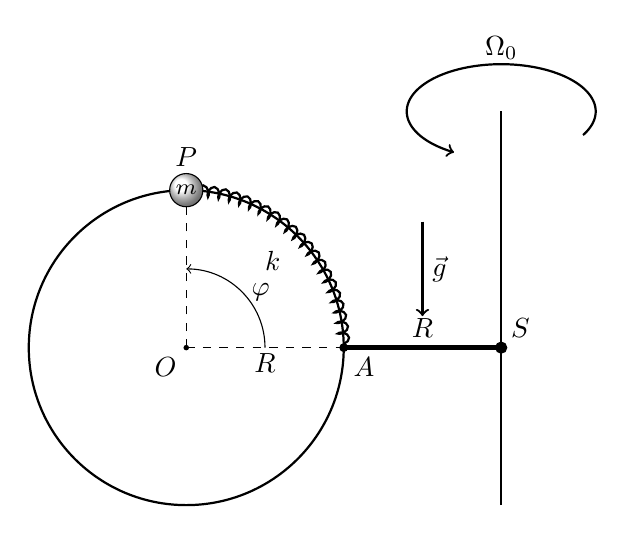
\begin{tikzpicture}[scale=2]
  % Radius
  \def\R{1}

  \coordinate (O) at (0,0);
  \coordinate (A) at (0,\R);
  \coordinate (P) at (\R,0);

  % Circle
  \draw[thick] (0,0) circle(\R);

  % Axes / radius lines
  \draw[dashed] (0,0) -- (0,\R);          % OA
  \draw[dashed] (0,0) -- (\R,0);          % OP

  % Points
  \fill (0,0) circle (0.5pt) node[below left] {$O$};
  \fill (0,\R) circle (1pt) node[above=5pt] {$P$};
 
  \fill (\R,0) circle (0.8pt) node[below right] {$A$};
  
        \draw[->] (0.5, 0) arc (0:90:0.5) node[midway, right] {$\varphi$};

  % Radius label
  \node at (0.5,-0.1) {$R$};
  \node[above] at (1.5*\R,0) {$R$};
  \filldraw (2*\R,0) circle (1pt) node[above right] {$S$};

  % Spring along arc from A to P (quarter circle, clockwise)
  \draw[decoration={coil, aspect=0.5, segment length=4pt, amplitude=2pt},
        decorate, thick] 
        (0,\R) arc[start angle=90, end angle=0, radius=\R];

  % Label for spring constant
  \node at (0.55,0.55) {$k$};

  
 \shadedraw[ball color=white] (0, \R) circle (3pt) node[font=\footnotesize] {$m$};
  % Horizontal bar from P to O (thick)
  \draw[line width=2pt] (\R,0) -- (2*\R,0);

  % Gravity vector
  \draw[->, thick] (1.5*\R,0.8) -- ++(0,-0.6);
  \node[right] at (1.5*\R,0.5) {$\vec{g}$};


 \draw[-,thick] (2,-1)--(2,1.5); 
    \begin{scope}[shift={(2,1.5)}, rotate=0]
    \draw[->,thick] 
      plot[domain=-30:240,variable=\t,smooth,samples=100] 
      ({0.6*cos(\t)}, {0.3*sin(\t)});
    \node at (0,0.4) {$\Omega_0$};
  \end{scope}

\end{tikzpicture}
    \caption{Sistema de anillo sobre aro circular giratorio con vínculo elástico.}
    \label{fig:anillo_aro}
\end{figure}

% --- SOLUCIÓN ---------------------------------------------------------------
\begin{solucion}{Anillo en aro circular con resorte}

\textbf{Marcos de referencia y Sistemas de Coordenadas}
\begin{itemize}
    \item $\mathcal{N}$: suelo (inercial) $\longrightarrow\{\vec{e}_x;\vec{e}_y;\vec{e}_z\}$, con origen en $S$ (punto del eje de giro a la altura de $O$).
    \item $\mathcal{A}$: aro $\longrightarrow\{\vec{e}_r;\vec{e}_\theta;\vec{e}_z\}$ (cilíndrica fija en el aro, con $\vec{e}_r$ horizontal desde el eje hacia el centro del aro).
    \item $\mathcal{B}$: marco imaginario orientado desde $O$ (centro del aro) hacia el anillo $P$ $\longrightarrow\{\vec{E}_r;\vec{E}_\varphi;\vec{e}_\theta\}$ en el plano del aro.
\end{itemize}

\begin{center}
\begin{tikzpicture}[>=Latex, scale=1.3]
    % --- PARÁMETROS ---
    \def\R{1.6}     % radio del aro [u]
    \def\ph{50}     % ángulo varphi [°]

    % --- EJE Y BARRA ---
    \draw[thick] (0,-1.5*\R) -- (0,1.7*\R);
    \draw[->, thick] (0,1.5*\R) -- (0,1.7*\R) node[above] {$\Omega_0$};
    \draw[line width=2pt] (0,0) -- (\R,0);
    \filldraw (0,0) circle (1.2pt) node[below left] {$S$};

    % --- ARO ---
    \coordinate (C) at (2*\R,0);
    \coordinate (A) at (\R,0);
    \coordinate (M) at ({2*\R-\R*cos(\ph)},{\R*sin(\ph)});
    \draw[thick] (C) circle (\R);
    \draw[dashed, gray] (C) -- (A);
    \draw[decoration={coil, aspect=0.5, segment length=3pt, amplitude=1.6pt}, decorate, thick]
        (A) arc (180:{180-\ph}:\R);
    \filldraw (C) circle (1pt) node[below right] {$O$};
    \filldraw (A) circle (1.2pt) node[below left] {$A$};
    \shadedraw[ball color=gray!30] (M) circle (3.5pt) node[above left] {$P$};

    % --- BASES ---
    \draw[azul, ultra thick, -{Latex}] (C) -- ++(0.9,0) node[right] {$\vec{e}_r$};
    \draw[azul, ultra thick, -{Latex}] (C) -- ++(0,0.9) node[right] {$\vec{e}_z$};
    \draw[myred, ultra thick, -{Latex}] (C) -- ({2*\R-0.9*cos(\ph)},{0.9*sin(\ph)}) node[below left, xshift=1pt, yshift=2pt] {$\vec{E}_r$};
    \draw[myred, ultra thick, -{Latex}] (M) -- ++({90-\ph}:0.9) node[above right] {$\vec{E}_\varphi$};
    \draw[->] ($(C)+(180:0.5)$) arc (180:{180-\ph}:0.5);
    \node at ({2*\R-0.75*cos(\ph/2)},{0.75*sin(\ph/2)-0.05}) {$\varphi$};
\end{tikzpicture}
\end{center}

\begin{equation*}
\begin{split}
    \vec{e}_r&=\cos(\Omega_0 t)\vec{e}_x+\sin(\Omega_0 t)\vec{e}_y\\
    \vec{e}_\theta&=-\sin(\Omega_0 t)\vec{e}_x+\cos(\Omega_0 t)\vec{e}_y\\
    \vec{E}_r&=-\cos\varphi\,\vec{e}_r+\sin\varphi\,\vec{e}_z\\
    \vec{E}_\varphi&=\sin\varphi\,\vec{e}_r+\cos\varphi\,\vec{e}_z
\end{split}
\end{equation*}

\textbf{Velocidad angular del aro}\\
$$\velang{N}{A}=\Omega_0\vec{e}_z\qquad\accang{N}{A}=\vec{0}$$

\subsubsection*{Cinemática de la partícula}
\textbf{Posición}\\
Como siempre, para obtener la velocidad respecto a un marco inercial partimos de la posición del anillo, medida desde un punto que no se mueve ($S$):
\begin{align*}
    \vec{r}_P &= 2R\,\vec{e}_r + R\,\vec{E}_r \\
              &= 2R\,\vec{e}_r + R\left[ -\cos\varphi\,\vec{e}_r + \sin\varphi\,\vec{e}_z \right] \\
              &= R\left(2 - \cos\varphi\right)\vec{e}_r + R\sin\varphi\,\vec{e}_z
\end{align*}

\textbf{Velocidad}\\
La velocidad es la derivada temporal de la posición:
\begin{align*}
\der{\vec{r}_P}{N}{} &= R \sin\varphi\,\dot{\varphi}\,\vec{e}_r + R(2 - \cos\varphi)\der{\vec{e}_r}{N}{} + R \cos\varphi\,\dot{\varphi}\,\vec{e}_z
\end{align*}

\patotruco{Aquí no hace falta escribir el teorema del transporte completo: como $\vec{e}_r$ y $\vec{e}_\theta$ solo giran en torno a $\vec{e}_z$ con velocidad angular $\Omega_0$, el trucazo es derivar $\vec{e}_r\to\Omega_0\vec{e}_\theta$ y $\vec{e}_\theta\to-\Omega_0\vec{e}_r$ (la demostración está en la Ayudantía 5).}

Derivadas temporales de $\vec{e}_r$ y $\vec{e}_\theta$:
$$\transport{\vec{e}_r}{N}{A}=\Omega_0\vec{e}_z\times\vec{e}_r=\Omega_0\vec{e}_\theta$$
$$\transport{\vec{e}_\theta}{N}{A}=\Omega_0\vec{e}_z\times\vec{e}_\theta=-\Omega_0\vec{e}_r$$
y finalmente
$$\marc{\vec{v}_P}{N}= R \sin\varphi\,\dot{\varphi}\,\vec{e}_r + R(2 - \cos\varphi)\,\Omega_0\,\vec{e}_\theta + R \cos\varphi\,\dot{\varphi}\,\vec{e}_z$$

\textbf{Aceleración}\\
Al igual que antes, derivamos la velocidad:
\begin{align*}
\marc{\vec{a}_P}{N}=\der{\vec{v}_P}{N}{} &= R \left[
\left( \ddot{\varphi} \sin\varphi + \dot{\varphi}^2 \cos\varphi - (2 - \cos\varphi) \Omega_0^2 \right) \vec{e}_r \right. \\
&\quad + \left(2 \dot{\varphi} \sin\varphi\, \Omega_0 \right) \vec{e}_\theta \\
&\quad + \left. \left( \ddot{\varphi} \cos\varphi - \dot{\varphi}^2 \sin\varphi \right) \vec{e}_z \right]
\end{align*}

\subsubsection*{Cinética}
\textbf{Diagrama de cuerpo libre}\\
Siempre se parte por un DCL, vista del plano $\vec{e}_r$-$\vec{e}_z$ (la normal $\vec{N}_\theta$ sale del plano):
\begin{center}
\begin{tikzpicture}[>=Latex, scale=1.0]
    \def\ph{50}
    \coordinate (M) at (0,0);
    \draw[->, thick, myred] (M) -- ++({180-\ph}:1.3) node[above left] {$\vec{N}_r$};
    \draw[->, thick, myred] (M) -- ++({270-\ph}:1.1) node[below left] {$\vec{F}_s$};
    \draw[->, thick, myred] (M) -- ++(0,-1.2) node[below] {$\vec{F}_g$};
    \shadedraw[ball color=gray!30] (M) circle (4pt);
    \node[above right] at (M) {$m$};
    \node at (1.3,0.9) {$\vec{N}_\theta$};
    \draw (1.8,0.9) circle (0.12); \fill (1.8,0.9) circle (1pt);
\end{tikzpicture}
\end{center}

Después del DCL se caracteriza cada fuerza vectorialmente. La fuerza de un resorte curvo tiene la dirección tangente de la curva en la que está contenido, en este caso $\vec{E}_\varphi$:
$$\vec{F}_s=-k(\ell-\ell_0)\vec{e}_t=-k(R\varphi-\ell_0)\vec{E}_{\varphi}=-k(R\varphi-\ell_0)\left(\sin\varphi\,\vec{e}_r+\cos\varphi\,\vec{e}_z\right)$$
$$\vec{F}_g=-mg\,\vec{e}_z$$
Al igual que en otros problemas, las direcciones de las normales son las direcciones normal y binormal de la curva:
$$\vec{N}_r=N_r\vec{E}_r=N_r\left( -\cos\varphi\,\vec{e}_r + \sin\varphi\,\vec{e}_z \right)$$
$$\vec{N}_\theta=N_\theta\vec{e}_\theta$$

\patoojo{El resorte curvo no tira en línea recta hacia $A$: su fuerza es tangente al aro y su largo es el arco $\ell=R\varphi$ (no la cuerda).}

\textbf{Ecuación diferencial}\\
Se plantea la segunda ley de Newton $\sum\vec{F}_{ext}=m\marc{\vec{a}_P}{N}$, proyectada en $\vec{e}_r$, $\vec{e}_\theta$ y $\vec{e}_z$:
\begin{align*}
-k(R\varphi-\ell_0)\sin\varphi - N_r\cos\varphi &= Rm \left( \ddot{\varphi} \sin\varphi + \dot{\varphi}^2 \cos\varphi - (2 - \cos\varphi) \Omega_0^2 \right)\\
N_\theta &= Rm \cdot 2 \dot{\varphi} \sin\varphi\, \Omega_0 \\
N_r\sin\varphi - mg - k(R\varphi - \ell_0)\cos\varphi &= Rm \left( \ddot{\varphi} \cos\varphi - \dot{\varphi}^2 \sin\varphi \right)
\end{align*}
Ignoramos la segunda ecuación, ya que no contiene $\ddot{\varphi}$.

\textbf{Paso 1: despejar $N_r$ de la primera ecuación.}
$$N_r = \frac{ -Rm \left( \ddot{\varphi} \sin\varphi + \dot{\varphi}^2 \cos\varphi - (2 - \cos\varphi) \Omega_0^2 \right) - k(R\varphi - \ell_0)\sin\varphi }{ \cos\varphi }$$

\textbf{Paso 2: sustituir $N_r$ en la tercera ecuación.}
\begin{multline*}
\left( \frac{ -Rm \left( \ddot{\varphi} \sin\varphi + \dot{\varphi}^2 \cos\varphi - (2 - \cos\varphi) \Omega_0^2 \right) - k(R\varphi - \ell_0)\sin\varphi }{ \cos\varphi } \right)\sin\varphi\\
- mg - k(R\varphi - \ell_0)\cos\varphi = Rm \left( \ddot{\varphi} \cos\varphi - \dot{\varphi}^2 \sin\varphi \right)
\end{multline*}

\textbf{Paso 3: expandir el lado izquierdo.}
\begin{multline*}
\frac{ -Rm \ddot{\varphi} \sin^2\varphi - Rm \dot{\varphi}^2 \cos\varphi\sin\varphi + Rm(2 - \cos\varphi) \Omega_0^2 \sin\varphi - k(R\varphi - \ell_0)\sin^2\varphi }{\cos\varphi}\\
- mg - k(R\varphi - \ell_0)\cos\varphi = Rm \ddot{\varphi} \cos\varphi - Rm \dot{\varphi}^2 \sin\varphi
\end{multline*}

\textbf{Paso 4: agrupar los términos con $\ddot{\varphi}$.}
$$\ddot{\varphi} \left( -Rm \left( \frac{\sin^2\varphi}{\cos\varphi} + \cos\varphi \right) \right)
= -Rm \ddot{\varphi} \cdot \frac{ \sin^2\varphi + \cos^2\varphi }{ \cos\varphi }
= -Rm \ddot{\varphi} \cdot \frac{1}{\cos\varphi}$$

\textbf{Paso 5: despejar $\ddot{\varphi}$.}\\
Multiplicamos ambos lados por $-\cos\varphi$ y el resultado es:
\respuesta{$\displaystyle \ddot{\varphi} = \frac{k(R\varphi - \ell_0) + mg \cos\varphi - Rm(2 - \cos\varphi)\, \Omega_0^2 \sin\varphi}{Rm}$}

\end{solucion}

\subsubsection{Partícula en ranura de disco giratorio}

Una partícula de masa $m$ se desliza dentro de una ranura recta en un disco rígido sin masa. La ranura está llena de un fluido que genera fricción en el movimiento de la partícula, cuyo coeficiente de fricción es $\nu$. El disco gira en el plano vertical con velocidad angular constante $\Omega$ en torno a un eje que pasa por el punto $O$, como se muestra en la Figura \ref{fig:disco_ranura}. Además, la ranura es ortogonal al diámetro del disco que contiene el punto $O$. Unido a la partícula hay un resorte lineal con constante de resorte $K$ y largo natural $\ell_0$. 

Utilizando el análisis de mecánica racional, realice lo siguiente:

\begin{enumerate}
    \item Defina los marcos de referencia y sistemas de coordenadas (fijo y móvil).
    \item Determine el vector posición, velocidad y aceleración de la partícula respecto al suelo.
    \item Identifique todas las fuerzas que actúan sobre la partícula (incluyendo la fuerza de fricción viscosa $\vec{F}_v = -\nu \vec{v}_{rel}$).
    \item Determine la ecuación diferencial de movimiento de la partícula en términos de la variable $x$.
\end{enumerate}

\begin{figure}[!ht]
    \centering
    \begin{tikzpicture}[>=Latex, scale=1.8]
        % --- Parámetros ---
        \def\ang{40}      % Ángulo Omega*t
        \def\distA{2}   % Distancia 'a' desde O al centro de la ranura
        \def\xPos{0.4}    % Posición x de la partícula respecto al centro
        \def\Rdisk{2.0}   % Radio visual del disco

        % --- Coordenadas ---
        \coordinate (O) at (0,0);
        % Dirección del diámetro (a lo largo de 'a')
        \coordinate (M) at ({\distA*sin(\ang)}, {-\distA*cos(\ang)});
        
        
        % --- 2. Soporte en O ---
        \begin{scope}
            \clip (-0.8,0.4) rectangle (0.4,-0.4);
            \fill[pattern=north east lines] (-0.3,0.1) rectangle (0.3,0.3);
            \filldraw[color=gris1!60] (0.2,0.1) arc (0:-180:0.2)--cycle;
            \draw[] (0.2,0.1) arc (0:-180:0.2)--cycle;
            \draw (-0.3,0.1) -- (0.3,0.1);
            
        \end{scope}
        % --- 1. Disco ---
        \shadedraw[inner color=white, outer color=gris1!20, draw=black, thick] (M) circle (\Rdisk);
        \filldraw (O) circle (1.5pt) node[below left] {$O$};
        
        % --- 3. Líneas de referencia ---
        \draw[dashed, gris1!60] (O) -- (0,-2.2);
        \draw[thick] (O) -- (M) node[midway, above right] {$a$};
        
        % Ángulo Omega*t
        \draw[->, azul] (0,-0.6) arc (270:{270+\ang}:0.6);
        \node[azul] at (0.2, -0.8) {$\Omega t$};

        % --- 4. Ranura y Partícula ---
        % Rotamos para dibujar la ranura perpendicular a OM
        \begin{scope}[shift={(M)}, rotate={\ang}]
            % Ranura (rectángulo)
            \draw[thick, fill=white] (-1, -0.2) rectangle (1, 0.2);
            
            % Eje x
            \draw[|->, thin] (0, -0.4) -- (0.8, -0.4) node[right] {$x$};
            \draw[|-|, thin] (-1, -0.4) --(0, -0.4) node[midway, below right] {$\ell_0$};
            

            % Resorte (desde Q a P)
            \draw[decoration={coil, segment length=4pt, amplitude=3pt}, decorate] 
                (-1, 0) -- (\xPos, 0) node[midway, right] {$K$};
            \filldraw (-1,0) circle (1pt) node[below] {$Q$};
            
            % Partícula P
            \shadedraw[ball color=gris1!20] (\xPos, 0) circle (4pt) node[above right, xshift=2pt] {$P$};
            \node[font=\footnotesize] at (\xPos, 0) {$m$};

        \end{scope}

        % --- 5. Gravedad ---
        \draw[->, thick, myred] (3.5, -0.5) -- (3.5, -1.3) node[midway, right] {$\vec{g}$};

    \end{tikzpicture}
    \caption{Esquema de una partícula con fricción viscosa y resorte en un disco rotatorio.}
    \label{fig:disco_ranura}
\end{figure}
\subsubsection{Partícula en superficie de un cono}

Una partícula $P$ de masa $m$ se mueve sin roce sobre la superficie exterior de un cono de ángulo $\phi = \pi/4$. El sistema se encuentra en el espacio profundo (sin gravedad). La partícula comienza su movimiento a una distancia $r_0$ del vértice, con una velocidad inicial perpendicular al eje $\vec{e}_z$ y una velocidad angular $\dot{\theta}(t_0) = \omega_0$. Además de la fuerza normal, existe una fuerza de atracción central ejercida por el eje $\vec{e}_z$ sobre la partícula:
\[ \vec{f} = -\frac{B}{\rho^2} \vec{e}_\rho \]
donde $B$ es una constante conocida y $\rho$ es la coordenada radial cilíndrica. Considerando el origen en el vértice del cono, realice lo siguiente:

\begin{enumerate}
    \item Defina los marcos de referencia y sistemas de coordenadas (esféricas y cilíndricas) adecuados.
    \item Encuentre la velocidad angular $\dot{\theta}$ de $P$ en función de la coordenada esférica $r$.
    \item Determine si la fuerza $\vec{f}$ es o no conservativa.
    \item Escriba la energía mecánica total en términos de $\dot{r}$ y $r$.
    \item Analice si existen soluciones donde la coordenada $r$ esté acotada entre dos valores, $r_{min}$ y $r_{max}$.
\end{enumerate}

\begin{figure}[!ht]
    \centering
    \begin{tikzpicture}[>=Latex, scale=1.5]
        % --- Parámetros ---
        \def\Rbase{2}
        \def\Hcone{2}
        \def\ang{45} % pi/4

        % --- 1. Dibujo del Cono ---
        % Elipse de la base (atrás)
        \draw[dashed, gray] (\Rbase, 0) arc (0:180:{\Rbase} and 0.6);
        % Superficie lateral
        \draw[thick] (-\Rbase, 0) -- (0, \Hcone) -- (\Rbase, 0);
        % Elipse de la base (adelante)
        \draw[thick] (-\Rbase, 0) arc (180:360:{\Rbase} and 0.6);

        % --- 2. Ejes y Ángulo ---
        \draw[->, dashed] (0, \Hcone) -- (0, -0.5) node[below] {$\vec{e}_z$};
        \draw[dashed] (0, \Hcone) -- +(0.8, -0.8);
        \draw[thin] (0, \Hcone-0.4) arc (270:315:0.4);
        \node at (0.2, \Hcone-0.6) {$\frac{\pi}{4}$};

        % --- 3. Partícula y Vectores ---
        % Posición de la partícula P
        \coordinate (V) at (0, \Hcone); % Vértice
        \coordinate (P) at (1.2, {\Hcone - 1.2}); % Punto en la superficie
        
        \filldraw[shading=ball, ball color=black] (P) circle (2.5pt) node[right, xshift=3pt] {$P$};
        
        % Vector e_r (A lo largo del cono)
        \draw[->, thick] (P) -- +(135:-0.8) node[right] {$\vec{e}_r$};
        % Vector e_phi (Perpendicular a la superficie)
        \draw[->, thick] (P) -- +(45:0.8) node[right] {$\vec{e}_\phi$};
        
        % Líneas auxiliares para rho
        \draw[dashed, gray] (P) -- (0, {\Hcone - 1.2});
        \node[above] at (0.6, {\Hcone - 1.2}) {$\rho$};

    \end{tikzpicture}
    \caption{Partícula $P$ en movimiento sobre la superficie de un cono bajo una fuerza central atractiva.}
    \label{fig:cono_particula}
\end{figure}
\subsubsection{Masa y resorte en el borde de una piscina}

Considere un sistema compuesto por un resorte y una masa que se encuentran al borde de una piscina muy profunda, como se indica en la Figura \ref{fig:piscina}. El resorte es de largo natural $\ell_0$ y constante elástica $k$. A éste se fija una pared móvil de masa despreciable. El sistema se prepara de tal modo que la partícula puntual de masa $m$ se coloca junto a esta pared en su posición de compresión máxima, es decir en $x = -\ell_0$, y se suelta desde el reposo.

\begin{enumerate}
    \item ¿Cuál es la condición que asegura que la masa $m$ se moverá desde $x = -\ell_0$?
    \item Encuentre el valor máximo de $\mu_d$ que permita a la masa llegar al borde de la piscina ($x = 0$) con velocidad no nula. Entregue el valor de esta velocidad.
    \item Una vez que entra a la piscina ($x > 0$), la masa experimenta una fuerza de roce viscoso lineal de constante $\gamma$. Suponga que no hay fuerza de empuje. Determine el alcance máximo y su velocidad límite.
\end{enumerate}

\begin{figure}[htbp]
    \centering
    \begin{tikzpicture}[>=Latex, scale=1.5]
        % --- Parámetros ---
        \def\Lzero{1.8} % Longitud L0
        
        % --- 1. El Suelo y la Piscina ---
        % Suelo (izquierda)
        \fill[gray!20] (-2.5, -2) rectangle (0, 0);
        \draw[thick] (-2.5, 0) -- (0, 0);
        \draw[pattern=north east lines, pattern color=gray!50] (-2.5, -2) rectangle (0, 0);
        
        % Piscina (derecha)
        \fill[blue!5] (0, -2) rectangle (2.5, 0);
        \draw[blue!40] (0, 0) -- (2.5, 0);
        % Líneas de agua
        \foreach \y in {-0.3, -0.7, -1.1, -1.5} {
            \draw[blue!30, thin] ({0.2-0.1*rand}, \y) -- ({2.3+0.1*rand}, \y);
        }
        \node[blue] at (0.5, -1) {$\gamma$};

        % --- 2. Ejes de Coordenadas ---
        \draw[->, thick] (-2.5, 0) -- (2.5, 0) node[right] {$x$};
        \draw[->, thick] (0, 0) -- (0, 1.2) node[above] {$y$};

        % --- 3. El Mecanismo (Muelle y Masa) ---
        % Pared fija
        \fill[gray!60] (-2.5, 0) rectangle (-2.2, 0.5);
        \draw[thick] (-2.2, 0) -- (-2.2, 0.5);
        
        % Resorte
        \draw[decoration={aspect=0.3, segment length=3pt, amplitude=3pt, coil}, decorate] 
            (-2.2, 0.25) -- (-\Lzero+0.2, 0.25);
        
        % Masa P
        \shadedraw[ball color=gray!80] (-\Lzero+0.2, 0.25) circle (7pt);
        \filldraw (-\Lzero+0.2, 0.25) circle (1pt); % centro
        
        % Cota L0
        \draw[|<->|] (-2.2, 0.7) -- (0, 0.7) node[midway, fill=white] {$\ell_0$};

        % --- 4. Traectoria de caída ---
        \draw[dashed, ->, gray] (0,0.15) parabola (1.8, -2);

        % --- 5. Etiquetas de coeficientes ---
        \node at (-1, -0.3) {$\mu_e, \mu_d$};
        \draw[->, thick] (1.2, 0.8) -- (1.2, 0.3) node[right] {$\mathbf{g}$};

    \end{tikzpicture}
    \caption{Sistema masa-resorte en el borde de una piscina con rozamiento seco y viscoso.}
    \label{fig:piscina}
\end{figure}
\subsubsection{Aro deslizante en brazo giratorio}

Un aro de masa $m$ se desliza sin fricción a lo largo de un brazo rígido sin masa de longitud variable. El brazo está articulado en uno de sus extremos en el punto $O$, el cual se encuentra en un eje vertical que gira con una velocidad angular constante $\Omega$. Además, el aro está unido a un resorte lineal con constante de resorte $K$ y largo natural $r_0$ conectado al punto $O$. El brazo puede girar libremente en el plano vertical. Utilizando las coordenadas $r$ (distancia al origen) y $\theta$ (ángulo con la vertical), realice lo siguiente:

\begin{enumerate}
    \item Defina los marcos de referencia y sistemas de coordenadas adecuados.
    \item Determine las expresiones para la energía cinética y potencial del sistema.
    \item Utilizando el formalismo de Lagrange, determine el sistema de dos ecuaciones diferenciales de movimiento para las variables $r$ y $\theta$.
\end{enumerate}

\begin{figure}[!ht]
    \centering
    \begin{tikzpicture}[>=Latex, scale=1.5]
        % --- Parámetros ---
        \def\ang{35} % Ángulo theta
        \def\rPos{2.2} % Posición r del aro

        % --- 1. Eje de Rotación ---
        \draw[dashed, thick] (0, 0.5) -- (0, -3.5);
        \draw[->, thick] (-0.3, 0.4) arc (180:450:0.3 and 0.1);
        \node[left] at (-0.3, 0.4) {$\Omega$};

        % Soporte O
        \fill[pattern=north east lines] (-0.3, 0) rectangle (0.3, 0.3);
        \draw[thick] (-0.3, 0) -- (0.3, 0);
        
        % --- 2. El Brazo y el Ángulo ---
        \begin{scope}[rotate=\ang]
            % El brazo
            \draw[line width=4pt, line cap=round] (0,0) -- (0, -3.2);
            \draw[line width=2.5pt, gray!60, line cap=round] (0,0) -- (0, -3.2);
            
            % El resorte
            \draw[decoration={aspect=0.3, segment length=3pt, amplitude=3.5pt, coil}, decorate] 
                (0,0) -- (0, -\rPos);
            \node[above right] at (0, -\rPos/2) {$K$};

            % El Aro (Masa m)
            \shadedraw[ball color=gray!30] (0, -\rPos) circle (0.1) node[font=\footnotesize] {$m$};
            
            % Cota r
            \draw[|<->|] (0.4, 0) -- (0.4, -\rPos) node[midway, above right] {$r$};
        \end{scope}

        % --- 3. Ángulo Theta ---
        \draw[dashed, gray] (0,0) -- (0, -1.5);
        \draw[->] (0, -0.8) arc (270:{270+\ang}:0.8);
        \node at (0.2, -1.0) {$\theta$};

        % --- 4. Articulación y Gravedad ---
        \filldraw[fill=gray!80] (0,0) circle (2pt) node[below left, xshift=-3pt] {$O$};
        \draw[->, thick] (1.7, -0.5) -- (1.7, -1.2) node[right] {$\mathbf{g}$};

    \end{tikzpicture}
    \caption{Sistema de un aro deslizante sobre un brazo rígido en rotación con vínculo elástico.}
    \label{fig:aro_brazo}
\end{figure}
% =========================================================================
% Capítulo 2: Cinética de la partícula
% Tema 01: Dinámica de la partícula
% Problema 09: Abrazadera en varilla horizontal con anclaje móvil
% Origen: Ayudantía 27, 2026
% =========================================================================
\subsubsection{Abrazadera en varilla horizontal con anclaje móvil}

Una abrazadera $P$ de masa $m$ desliza sin roce a lo largo de una varilla rígida, horizontal y fija (Figura \ref{fig:abrazadera}). Está unida a un resorte lineal de constante $k$ y largo natural $l_0$, cuyo otro extremo $Q$ se mueve con una ley prescrita $q(t)$. Tanto $q$ como la posición $x$ de la abrazadera se miden desde la pared izquierda, y $P$ se mantiene a la derecha de $Q$. No hay gravedad.

Resuelva usando trabajo y energía:
\begin{enumerate}
    \item Trate la fuerza del resorte como una fuerza externa (no conservativa) y obtenga la ecuación diferencial de $x(t)$ con el teorema de trabajo y energía.
    \item Trate el resorte como conservativo, con energía potencial $V(x,t)$. Calcule $dE/dt$ para $E=T+V$ y obtenga nuevamente la ecuación diferencial.
    \item Determine la potencia que debe entregar el mecanismo que mueve $Q$ y compárela con $dE/dt$.
\end{enumerate}

\begin{figure}[!ht]
    \centering
    \begin{tikzpicture}[>=Latex, scale=1.2]
        % --- PARÁMETROS ---
        \def\Lv{6.0}      % largo de la varilla [u]
        \def\xQ{1.9}      % posición del anclaje: q [u]
        \def\xP{4.5}      % posición de la abrazadera: x [u]

        % --- VARILLA Y PAREDES ---
        \draw[line width=4pt, gray!35] (0,0) -- (\Lv,0);
        \fill[pattern=north east lines] (-0.2,-0.45) rectangle (0,0.45);
        \draw[thick] (0,-0.45) -- (0,0.45);
        \draw[thick] (\Lv,-0.45) -- (\Lv,0.45);
        \fill[pattern=north east lines] (\Lv,-0.45) rectangle ({\Lv+0.2},0.45);

        % --- RESORTE, ANCLAJE Q Y ABRAZADERA P ---
        \draw[decorate, decoration={coil, aspect=0.4, segment length=3pt, amplitude=3pt}, thick] (\xQ,0) -- (\xP,0);
        \shadedraw[ball color=white!90] (\xQ,0) circle (0.13);
        \shadedraw[ball color=gray!30] (\xP,0) circle (0.13);
        \node[below=5pt] at (\xQ,0) {$Q$};
        \node[below=5pt] at (\xP,0) {$P$};
        \node[above=4pt] at ({(\xQ+\xP)/2},0) {$k$};
        \node[above=3pt, font=\small] at (\xP,0.02) {$m$};

        % --- COTAS ---
        \draw[|->, thick, gray] (0,0.75) -- (\xQ,0.75) node[midway, above] {$q(t)$};
        \draw[|-|, thick, gray] (\xQ,0.75) -- (\xP,0.75) node[midway, above] {$x-q$};
        \draw[|->, thick, gray] (0,-0.85) -- (\xP,-0.85) node[midway, below] {$x$};
        \draw[thin, gray] (\xQ,0.45) -- (\xQ,0.9);
        \draw[thin, gray] (\xP,-0.5) -- (\xP,-1.0);
    \end{tikzpicture}
    \caption{Abrazadera $P$ con anclaje móvil $Q$ y resorte lineal.}
    \label{fig:abrazadera}
\end{figure}

% --- SOLUCIÓN ---------------------------------------------------------------
\begin{solucion}{Abrazadera en varilla horizontal con anclaje móvil}

\textbf{Marcos de referencia y Sistemas de Coordenadas}\\
Basta un marco inercial fijo a la varilla, con $\vec{e}_x$ a lo largo de ella y origen en la pared izquierda.

\subsubsection*{Cinemática de la partícula}
Como $\vec{e}_x$ es constante, las posiciones se derivan directamente:
$$\vec{r}_P=x\vec{e}_x\qquad\vec{r}_Q=q\vec{e}_x\qquad\vec{v}_P=\dot{x}\vec{e}_x\qquad\vec{a}_P=\ddot{x}\vec{e}_x$$
El largo del resorte es $x-q$, su elongación es $\delta=x-q-l_0$ y su rapidez de deformación es $\dot\delta=\dot{x}-\dot{q}$. La abrazadera solo se traslada, sin rotar, así que
$$T=\frac{1}{2}m\dot{x}^2$$

\subsubsection*{Cinética}
Sobre la abrazadera actúan el resorte y la reacción de la varilla. La reacción es perpendicular a $\vec{e}_x$, o sea a la velocidad, y no trabaja: la única fuerza que trabaja es la del resorte.

\textbf{Diagrama de cuerpo libre}
\begin{center}
    \begin{tikzpicture}[>=Latex, scale=1.2]
        \draw[line width=4pt, gray!35] (-1.5,0) -- (2.5,0);
        \shadedraw[ball color=gray!30] (0,0) circle (0.14);
        \draw[->, thick, myred] (0,0) -- (-1.2,0) node[midway, above] {$k\delta$};
        \draw[->, thick, myred] (0,0) -- (0,0.9) node[above] {$N$};
        \draw[->, thick, azul] (0,-0.3) -- (1.2,-0.3) node[midway, below] {$\dot{x}$};
    \end{tikzpicture}
\end{center}
La fuerza del resorte sobre $P$ vale $\vec{F}_s=-k\delta\,\vec{e}_x$ (en la figura, con $\delta>0$, tira hacia $Q$).

\textbf{1) Resorte como fuerza no conservativa}\\
La energía cinética cambia solo por la potencia que entrega el resorte:
$$\frac{dT}{dt}=\vec{F}_s\cdot\vec{v}_P\quad\Longrightarrow\quad m\dot{x}\ddot{x}=-k\left(x-q-l_0\right)\dot{x}$$
Simplificando $\dot{x}$ (distinto de cero mientras la abrazadera se mueve):
\respuesta{$\displaystyle m\ddot{x}+k\left(x-q-l_0\right)=0$}

\textbf{2) Resorte como fuerza conservativa}\\
Incluimos el resorte en el potencial. Como el anclaje se mueve, $V$ depende explícitamente del tiempo:
$$V(x,t)=\frac{1}{2}k\left(x-q(t)-l_0\right)^2$$
Entonces $E=T+V$ no se conserva: su variación es la derivada parcial del potencial respecto al tiempo,
$$\frac{dE}{dt}=\frac{\partial V}{\partial t}=-k\left(x-q-l_0\right)\dot{q}$$
Desarrollando el lado izquierdo,
$$m\dot{x}\ddot{x}+k\left(x-q-l_0\right)\left(\dot{x}-\dot{q}\right)=-k\left(x-q-l_0\right)\dot{q}$$
los términos con $\dot{q}$ se cancelan y queda $m\dot{x}\ddot{x}+k\left(x-q-l_0\right)\dot{x}=0$. Al simplificar $\dot{x}$ resulta la misma ecuación:
\respuesta{$\displaystyle m\ddot{x}+k\left(x-q-l_0\right)=0\quad\text{es decir}\quad m\ddot{x}+kx=k\left(q(t)+l_0\right)$}
Es un oscilador de frecuencia natural $\omega_n=\sqrt{k/m}$ forzado por el anclaje. En la variable $\delta$ queda $\ddot\delta+\omega_n^2\delta=-\ddot{q}$: lo que excita al resorte es la \emph{aceleración} de $Q$.

% NOTA PARA REVISIÓN (agente B): el ítem 3 (potencia del mecanismo) NO está resuelto en Ay27S.tex;
% el desarrollo de abajo es una derivación propia del agente, consistente con el dE/dt de arriba.
\textbf{3) Potencia del mecanismo que mueve $Q$}\\
El resorte tira de $Q$ con $+k\delta\,\vec{e}_x$ (hacia $P$), de modo que el mecanismo debe ejercer $-k\delta\,\vec{e}_x$ para imponer $q(t)$. Su potencia es
$$\mathcal{P}_{mec}=\left(-k\delta\,\vec{e}_x\right)\cdot\dot{q}\,\vec{e}_x=-k\left(x-q-l_0\right)\dot{q}$$
que coincide con $dE/dt=\partial V/\partial t$: la energía de $E=T+V$ varía solo por lo que entrega (o absorbe) el mecanismo que mueve $Q$.

\end{solucion}

\subsubsection{Partícula en resorte con anclaje móvil}

Una partícula de masa $m$ está unida a un resorte lineal con constante elástica $k$ y longitud natural $r_0$ El otro extremo del resorte está conectado a una abrazadera sin masa que se desliza sobre una guía horizontal sin fricción, cuyo desplazamiento $x(t)$ respecto a un origen fijo es conocido. Sabiendo que la gravedad actúa hacia abajo, se requiere analizar el comportamiento dinámico del sistema mostrado en la Figura \ref{fig:particula_resorte_movil}.

\begin{enumerate}
    \item Defina los marcos de referencia y sistemas de coordenadas adecuados.
    \item Determine y analice la cinemática de la partícula utilizando las variables $r$ y $\theta$.
    \item Determine y analice la cinética de la partícula para obtener las ecuaciones diferenciales de movimiento.
\end{enumerate}

\begin{figure}[!ht]
    \centering
    \begin{tikzpicture}[>=Latex, scale=1.5]
        % --- Parámetros de diseño ---
        \def\rL{3.0}      % Longitud del dibujo para r
        \def\ang{35}     % Ángulo theta
        \def\guideW{3.5}  % Ancho de la guía
        
        % --- Coordenadas ---
        \coordinate (Origin) at (-2, 0);       % Referencia fija
        \coordinate (O) at (0.5, 0);           % Posición de la abrazadera
        \coordinate (P) at ($(O) + ({\rL*sin(\ang)}, {-\rL*cos(\ang)})$); % Partícula
        
        % --- 1. Guía horizontal y soportes ---
        \draw[line width=3pt, black] (-\guideW, 0) -- (\guideW, 0);
        \draw[line width=2.5pt, gris1!40] (-\guideW, 0) -- (\guideW, 0);
        % Soporte Izquierdo
        \fill[pattern=north east lines] (-\guideW-0.3, -0.4) rectangle (-\guideW, 0.4);
        \draw[thick] (-\guideW, -0.4) -- (-\guideW, 0.4);
        % Soporte Derecho
        \fill[pattern=north east lines] (\guideW, -0.4) rectangle (\guideW+0.3, 0.4);
        \draw[thick] (\guideW, -0.4) -- (\guideW, 0.4);

        % --- 2. Abrazadera O ---
        \shadedraw[ball color=gris1!10, draw=black] (O) ellipse (0.15 and 0.15);
        \node[below left, xshift=-2pt] at (O) {$O$};
        \draw[black] (O) circle (0.15);

        % --- 3. Desplazamiento x(t) ---
        \draw[dashed, thin] (Origin) -- (Origin);
        \draw[dashed, thin] (Origin) -- ++(0, 0.8);
        \draw[dashed, thin] (O) -- ++(0, 0.8);
        \draw[|->, thick] ($(Origin)+(0,0.6)$) -- ($(O)+(0,0.6)$) node[midway, above] {$x(t)$};

        % --- 4. Resorte y Coordenadas ---
        % Línea de referencia vertical
        \draw[dashed, gris1!60] (O) -- ++(0, -3.5);
        
        % Resorte
        \draw[decoration={aspect=0.4, segment length=3mm, amplitude=3mm, coil}, decorate, thick] (O) -- (P);
        \node[left, xshift=-8pt] at ($(O)!0.5!(P)$) {$k$};

        % Ángulo theta
        \draw[->] (0.5, -0.8) arc (270:{270+\ang}:0.8);
        \node at (0.7, -1.0) {$\theta$};

        % Vector r (distancia)
        \draw[|<->|, thin] ($(O)+(0.4, 0.2)$) -- ($(P)+(0.4, 0.2)$) node[midway, above right] {$r$};

        % --- 5. Partícula P ---
        \shadedraw[ball color=gris1!30] (P) circle (0.2);
        \node at (P) {$m$};
        \node[right, xshift=10pt] at (P) {$P$};

        % --- 6. Vector de gravedad ---
        \draw[->, thick, myred] (-2.5, -1.5) -- (-2.5, -2.5) node[midway, left] {$\mathbf{g}$};

    \end{tikzpicture}
    \caption{Esquema de una partícula $m$ acoplada a un resorte con soporte móvil $x(t)$.}
    \label{fig:particula_resorte_movil}
\end{figure}

% =========================================================================
% Capítulo 2: Cinética de la partícula
% Tema 01: Dinámica de la partícula
% Problema 11: Collar en riel circular con resorte excéntrico
% Origen: Ayudantía 27, 2026
% =========================================================================
\subsubsection{Collar en riel circular con resorte excéntrico}

Un collar de masa $m$ desliza sin roce sobre un riel circular de radio $R$ contenido en un plano horizontal, como se muestra en la Figura \ref{fig:collar_riel}. El collar está unido a un punto fijo $A$ mediante un resorte de constante elástica $K$ y largo natural nulo. El punto $A$ está a una distancia $2R$ del centro $O$ del riel, sobre la recta horizontal de referencia. La posición del collar se mide con el ángulo $\phi$ desde esa recta, en sentido antihorario. No hay gravedad, y las condiciones iniciales son $\phi_0$ y $\dot\phi_0$.

Resuelva usando trabajo y energía:
\begin{enumerate}
    \item Obtenga la ecuación diferencial del movimiento de $\phi(t)$.
    \item Determine $\dot\phi$ como función de $\phi$.
    \item Calcule la fuerza de reacción del riel sobre el collar en función de $\phi$.
    \item Encuentre las posiciones de equilibrio, determine su estabilidad y la frecuencia de las oscilaciones pequeñas alrededor de la estable.
\end{enumerate}

\begin{figure}[!ht]
    \centering
    \begin{tikzpicture}[>=Latex, scale=1.5]
        % --- Parámetros ---
        \def\R{1.5}          % Radio del riel
        \def\ang{30}         % Ángulo phi
        \def\distA{2*\R}     % Distancia OA

        % --- 1. Riel Circular ---
        \draw[thick] (0,0) circle (\R);
        \draw[dashed] (-\distA-0.5, 0) -- (\R+0.5, 0); % Eje horizontal de referencia
        \filldraw (0,0) circle (1.5pt) node[below] {$O$};

        % --- 2. Punto Fijo A ---
        \coordinate (A) at (-\distA, 0);
        \fill[pattern=north east lines] (-\distA-0.3, -0.2) rectangle (-\distA, 0.2);
        \draw[thick] (-\distA, -0.2) -- (-\distA, 0.2);
        \filldraw (A) circle (2pt) node[below right] {$A$};

        % --- 3. Posición del Collar ---
        \coordinate (M) at ({\R*cos(\ang)}, {\R*sin(\ang)});
        
        % Radio R y Ángulo phi
        \draw[dashed] (0,0) -- (M);
        \draw[->] (0.6, 0) arc (0:\ang:0.6);
        \node at (0.8, 0.2) {$\phi$};
        \node at (0.4, 0.4) {$R$};

        % --- 4. Resorte ---
        \draw[decoration={aspect=0.3, segment length=3pt, amplitude=2.5pt, coil}, decorate] 
            (A) -- (M);
        \node[above] at ($(A)!0.5!(M)$) {$K$};

        % --- 5. Masa m (Collar) ---
        \shadedraw[ball color=gray!30] (M) circle (0.15);
        \node[above right] at (M) {$m$};

        % --- 6. Vector de Gravedad (indicativo de plano horizontal) ---
        % Nota: El enunciado dice sin gravedad, pero se incluye el vector 
        % tachado o lateral para cumplir con la regla de formato visual.
        %\draw[->, thick] (2, 1) -- (2, 0.5) node[midway, right] {$\mathbf{g}$};

    \end{tikzpicture}
    \caption{Diagrama de un collar de masa $m$ deslizando en un riel circular con vínculo elástico desde un punto exterior.}
    \label{fig:collar_riel}
\end{figure}

% --- SOLUCIÓN ---------------------------------------------------------------
% NOTA PARA REVISIÓN (agente B): el ítem 4 (equilibrios, estabilidad y frecuencia de pequeñas
% oscilaciones) NO está resuelto en Ay27S.tex ni en Ay3S.tex; se mantiene en el enunciado sin solución.
\begin{solucion}{Collar en riel circular con resorte excéntrico}

\textbf{Marcos de referencia y Sistemas de Coordenadas}\\
Lo primero, como en todo ejercicio, es definir los marcos de referencia.
\begin{itemize}
    \item $\mathcal{N}$: el suelo $\longrightarrow\{\vec{e}_x;\vec{e}_y;\vec{e}_z\}$
    \item $\mathcal{A}$: cilíndrico $OM$ $\longrightarrow\{\vec{e}_r;\vec{e}_\theta;\vec{e}_z\}$
\end{itemize}

\begin{center}
\begin{tikzpicture}[scale=0.8]
    \Polaresrtz{\phi}{e}{e}{azul}{myred}
    \node[below right] at (35:2) {$m$};
\end{tikzpicture}
\end{center}

\begin{equation*}
\begin{split}
    \vec{e}_r&=\cos\phi\,\vec{e}_x+\sin\phi\,\vec{e}_y\\
    \vec{e}_\theta&=-\sin\phi\,\vec{e}_x+\cos\phi\,\vec{e}_y\\
    \vec{e}_z&=\vec{e}_z
\end{split}
\end{equation*}

\subsubsection*{Cinemática de la partícula}
\textbf{Posición}\\
Como siempre, para obtener la velocidad de algún punto respecto a un marco de referencia inercial partimos por la posición; en este caso la de la masa $m$ es
$$\vec{r}_m=R\,\vec{e}_r$$

\textbf{Velocidad}\\
La velocidad es la derivada temporal de la posición:
$$\marc{\vec{v}_m}{N}=\der{\vec{r}_{m}}{N}=\der{(R\vec{e}_r)}{N}=R\der{\vec{e}_r}{N}{}$$

\patotruco{No es necesario usar el teorema del transporte completo: usamos el trucazo (la demostración está en la Ayudantía 5). Basta con derivar la base: $\dot{\vec{e}}_r=\dot\phi\,\vec{e}_\theta$ y $\dot{\vec{e}}_\theta=-\dot\phi\,\vec{e}_r$.}

Derivadas temporales de $\vec{e}_r$ y $\vec{e}_\theta$:
$$\transport{\vec{e}_r}{N}{A}=\dot\phi\vec{e}_z\times\vec{e}_r=\dot\phi\vec{e}_\theta$$
$$\transport{\vec{e}_\theta}{N}{A}=\dot\phi\vec{e}_z\times\vec{e}_\theta=-\dot\phi\vec{e}_r$$
y finalmente
$$\marc{\vec{v}_m}{N}=R\dot\phi\,\vec{e}_\theta$$

\textbf{Aceleración}\\
Al igual que antes, podemos simplemente derivar la velocidad:
% NOTA PARA REVISIÓN (agente B): el zip escribe +R*phi'^2 e_r; el signo correcto es -R*phi'^2 e_r
% (y es el que se usa más abajo en Newton). Se deja tal cual.
$$\marc{\vec{a}_m}{N}=\der{\marc{\vec{v}_m}{N}{}}{N}{}=\der{\left(R\dot\phi\,\vec{e}_\theta\right)}{N}{}=(R\dot\phi^2)\vec{e}_r+ R\ddot\phi\,\vec{e}_{\theta}$$

\subsubsection*{Cinética}
\textbf{Diagrama de cuerpo libre}\\
Siempre se parte por un DCL:
\begin{center}
\begin{tikzpicture}[>=Latex, scale=1.1]
    \def\R{1.5}
    \def\ang{35}
    \draw[thick] (0,0) circle (\R);
    \coordinate (A) at ({-2*\R},0);
    \coordinate (M) at ({\R*cos(\ang)},{\R*sin(\ang)});
    \filldraw (A) circle (1.5pt) node[below] {$A$};
    \filldraw (0,0) circle (1pt) node[below] {$O$};
    \draw[dashed, gray] (A) -- (M);
    \draw[->, very thick, orange!80!black] (M) -- ($(M)!0.45!(A)$) node[below, pos=0.9] {$\vec{F}_s$};
    \draw[->, very thick, violet!80!black] (M) -- ++(\ang:0.9) node[above right] {$\vec{N}$};
    \shadedraw[ball color=gray!30] (M) circle (4pt);
\end{tikzpicture}
\end{center}
Después del DCL se caracteriza cada fuerza vectorialmente:
$$\vec{F}_s=-K(\ell-\ell_0)\vec{u}_s;\quad \ell=\|R\vec{e}_r+2R\vec{e}_x\|;\quad\ell_0=0;\quad\vec{r}-\vec{r}_A=(R\vec{e}_r)-(-2R\vec{e}_x)$$
$$\vec{u}_s = \frac{\vec{r} - \vec{r}_A}{\left\lVert \vec{r} - \vec{r}_A \right\rVert}=\frac{R\vec{e}_r+2R\vec{e}_x}{\|R\vec{e}_r+2R\vec{e}_x\|}$$
$$\vec{F}_s=-K\|R\vec{e}_r+2R\vec{e}_x\|\frac{\vec{r} - \vec{r}_A}{\left\lVert \vec{r} - \vec{r}_A \right\rVert}=-K(R\vec{e}_r+2R\vec{e}_x)$$
En este caso tenemos dos normales, pero como el problema es 2D una de ellas desaparece, y la dirección se obtiene mediante intuición o matemáticamente con las coordenadas intrínsecas de la curva, en este caso un círculo:
$$\vec{N}=N\vec{e}_r$$

\textbf{Energía}\\
Si lo hacemos con energía tenemos
$$T=\frac{1}{2}m\left|\vec{v}_P\right|^2=\frac{1}{2}mR^2\dot\phi^2$$
El punto $A$ está fijo en $\vec{r}_A=-2R\,\vec{e}_x$. El vector que va de $A$ al collar es $R\vec{e}_r+2R\vec{e}_x$, y como $\vec{e}_x=\cos\phi\,\vec{e}_r-\sin\phi\,\vec{e}_\theta$,
$$\vec{r}_P-\vec{r}_A=R\left(1+2\cos\phi\right)\vec{e}_r-2R\sin\phi\,\vec{e}_\theta$$
$$\ell^2=R^2\left[\left(1+2\cos\phi\right)^2+4\sin^2\phi\right]=R^2\left(5+4\cos\phi\right)$$
Como el largo natural es nulo, la elongación es el propio $\ell$ y
$$V=\frac{1}{2}K\ell^2=\frac{1}{2}KR^2\left(5+4\cos\phi\right)$$
La conservación de la energía mecánica, con $\phi_0$ y $\dot\phi_0$ como condiciones iniciales, es
$$\frac{1}{2}mR^2\dot\phi^2+\frac{1}{2}KR^2\left(5+4\cos\phi\right)=\frac{1}{2}mR^2\dot\phi_0^2+\frac{1}{2}KR^2\left(5+4\cos\phi_0\right)$$
Derivando respecto al tiempo, $mR^2\dot\phi\ddot\phi-2KR^2\sin\phi\,\dot\phi=0$, y simplificando $mR^2\dot\phi$:
\respuesta{$\displaystyle \ddot\phi=\frac{2K}{m}\sin\phi$}

\textbf{Segunda ley de Newton}
$$\sum \vec{F} = m \vec{a}$$
$$\sum \vec{F} = \vec{N} + \vec{F}_s = \left[ N - KR(1 + 2\cos\phi) \right] \vec{e}_r + 2KR \sin\phi \, \vec{e}_\theta$$
$$\sum F_{\vec{e}_r} = N - KR(1 + 2\cos\phi) = m(-R\dot{\phi}^2)$$
$$\sum F_{\vec{e}_\theta} = 2KR \sin\phi = m(R\ddot{\phi})\quad\Longrightarrow\quad\ddot{\phi} - \frac{2K}{m} \sin\phi = 0$$
que coincide con lo obtenido por energía. De la ecuación en $\vec{e}_r$:
$$N = -mR\dot{\phi}^2 + KR(1 + 2\cos\phi)$$

\textbf{Fuerza de reacción en función de $\phi$}\\
Queremos la expresión en función de $\phi$, no de $\dot{\phi}$. De la segunda EDO tenemos $\ddot{\phi} = \frac{2K}{m} \sin\phi$. Usamos el truco
$$\ddot{\phi} = \frac{d\dot{\phi}}{dt} = \frac{d\dot{\phi}}{d\phi} \cdot \frac{d\phi}{dt} = \dot{\phi} \frac{d\dot{\phi}}{d\phi}$$
(que deja el diferencial en función de $\phi$). Sustituimos e integramos ambos lados:
$$\dot{\phi} \frac{d\dot{\phi}}{d\phi} = \frac{2K}{m} \sin\phi\quad\Longrightarrow\quad\int_{\dot{\phi}_0}^{\dot{\phi}} \dot{\phi} \, d\dot{\phi} = \int_{\phi_0}^{\phi} \frac{2K}{m} \sin\phi \, d\phi$$
$$\frac{\dot{\phi}^2}{2} - \frac{\dot{\phi}_0^2}{2} = -\frac{2K}{m} (\cos\phi - \cos\phi_0)$$
y reordenando:
\respuesta{$\displaystyle \dot{\phi}^2 = \dot{\phi}_0^2 + \frac{4K}{m} (\cos\phi_0 - \cos\phi)$}
Reemplazando en la ecuación de $N$:
% NOTA PARA REVISIÓN (agente B): en el zip el resultado final conserva -mR*phi'^2 (debería ser -mR*phi'_0^2
% tras sustituir). Se deja tal cual.
\begin{align*}
N &= -mR\left[ \dot{\phi}^2_0 + \frac{4K}{m}(\cos \phi_0 - \cos \phi) \right] + KR(1 + 2\cos\phi) \\
  &= -mR\dot{\phi}^2 - 4KR(\cos \phi_0 - \cos \phi) + KR(1 + 2\cos\phi) \\
  &= -mR\dot{\phi}^2 - 4KR\cos \phi_0 + 6KR\cos \phi + KR
\end{align*}
Por lo tanto, la fuerza de reacción ejercida sobre la partícula es:
\respuesta{$\displaystyle \vec{N} = \left[ -mR\dot{\phi}^2 - 4KR\cos \phi_0 + 6KR\cos \phi + KR \right] \vec{e}_r$}

\end{solucion}

% =========================================================================
% Capítulo 2: Cinética de la partícula
% Tema 01: Dinámica de la partícula
% Problema 12: Partícula en pista parabólica rotatoria
% Origen: Ayudantía 3, 2026
% =========================================================================
\subsubsection{Partícula en pista parabólica rotatoria}

Una partícula de masa $m$ se desliza sin fricción a lo largo de una pista en forma de parábola como se muestra en la \text{Figura \ref{fig:parabola_rotatoria}}. La ecuación que describe la geometría de la pista está dada por:
\[ y = \frac{r^2}{2a} \]
donde $a$ es una constante, $r$ es la distancia radial desde el eje vertical de simetría (punto $O$ al punto $B$), y $y$ es la distancia vertical desde el origen $O$ al punto $Q$. 

La partícula está unida a un resorte lineal de constante elástica $k$ y longitud natural $\ell_0$. El resorte se mantiene siempre alineado horizontalmente, conectando la partícula con un punto de unión libre de deslizarse a lo largo del eje vertical que pasa por el centro de la parábola. El sistema completo rota con una velocidad angular constante $\Omega$ alrededor de la dirección vertical. Considerando que la gravedad $\mathbf{g}$ actúa verticalmente hacia abajo, realice lo siguiente:

\begin{enumerate}
    \item Defina los marcos de referencia y sistemas de coordenadas adecuados para describir el movimiento en términos de la variable $r$.
    \item Analice la cinemática de la partícula, determinando el momento lineal y el momento angular respecto al punto $Q$.
    \item Analice la cinética de la partícula y determine la ecuación diferencial del movimiento en términos de la variable $r$.
\end{enumerate}

\begin{figure}[!ht]
    \centering
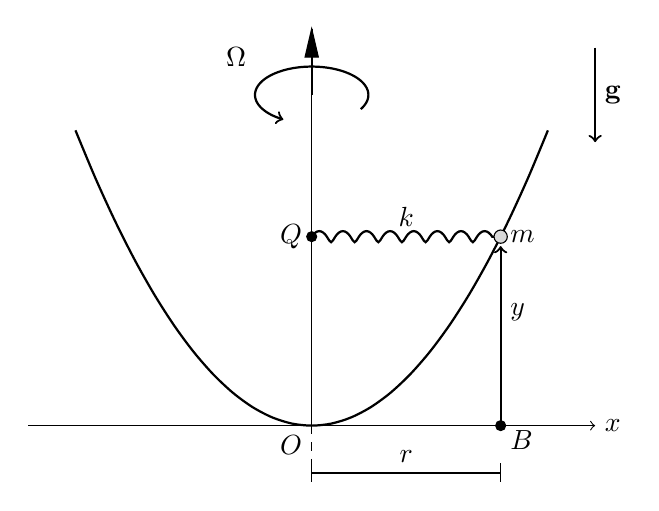
\begin{tikzpicture}[scale=1.2]
  % Axes
  \draw[->] (-3,0) -- (3,0) node[right] {$x$};
  \draw[-] (0,0) -- (0,4) ;

  % Origin
  \node[below left] at (0,0) {$O$};

  % Parabola
  \draw[domain=-2.5:2.5,smooth,variable=\x,thick] 
    plot ({\x},{0.5*\x*\x});

  % Dashed guides to Q
  \node[below, right] at (2,-0.15) {$B$};
    \filldraw[black] (2,0) circle (1.5pt);
  \draw[dashed] (0,0) -- (0,2) node[left] {$Q$};
    \filldraw[black] (0,2) circle (1.5pt);

  % Spring from Q to m
  \draw[decorate,decoration={coil,aspect=0.3, segment length=3mm, amplitude=2pt}, thick]
    (0,2) --node[midway,above] {$k$} (2,2);

  % Mass at end of spring
  \filldraw[fill=gray!30,draw=black] (2,2) circle (2pt);
  \node[right] at (2,2) {$m$};

  % Vertical arrow from parabola to mass: y
  \draw[->,thick] (2,0) -- (2,1.9);
  \node[right] at (2,1.2) {$y$};

  % Gravity arrow g
  \draw[->,thick] (3,4) -- (3,3);
  \node[right] at (3,3.5) {$\mathbf{g}$};

  \begin{scope}[shift={(0,3.5)}, rotate=0]
    \draw[->,thick] 
      plot[domain=-30:240,variable=\t,smooth,samples=100] 
      ({0.6*cos(\t)}, {0.3*sin(\t)});
    \node at (-0.8,0.4) {$\Omega$};
  \end{scope}
    % Axis stub and triangle tip
  \draw[thick] (0,3.5) -- (0,4.2);
  \draw[fill=black] (0,4.2) -- (-2pt,3.9) -- (2pt,3.9) -- cycle;

  %FLECHA r
  

\draw[-,dashed] (0,0)--(0,-0.5);
\draw[-,thick] (0,-0.5) -- node[midway, above] {$r$} (2,-0.5);
\draw (0,-0.4) -- (0,-0.6);
\draw (2,-0.4) -- (2,-0.6);

\end{tikzpicture}
    \caption{Diagrama de una partícula de masa $m$ en una pista parabólica rotatoria con vínculo elástico horizontal.}
    \label{fig:parabola_rotatoria}
\end{figure}

% --- SOLUCIÓN ---------------------------------------------------------------
\begin{solucion}{Partícula en pista parabólica rotatoria}

\textbf{Marcos de referencia y Sistemas de Coordenadas}\\
Lo primero, como en todo ejercicio, es definir los marcos de referencia.
\begin{itemize}
    \item $\mathcal{N}$: el suelo $\longrightarrow\{\vec{e}_x;\vec{e}_y;\vec{e}_z\}$
    \item $\mathcal{A}$: parábola $\longrightarrow\{\vec{e}_r;\vec{e}_\theta;\vec{e}_z\}$
\end{itemize}

\begin{center}
\begin{tikzpicture}[scale=0.8]
    \Polaresrtz{\Omega t}{e}{e}{azul}{myred}
    \node[above right] at (35:2) {$P$};
\end{tikzpicture}
\end{center}

\begin{equation*}
\begin{split}
    \vec{e}_r&=\cos(\Omega t)\vec{e}_x+\sin(\Omega t)\vec{e}_y\\
    \vec{e}_\theta&=-\sin(\Omega t)\vec{e}_x+\cos(\Omega t)\vec{e}_y\\
    \vec{e}_z&=\vec{e}_z
\end{split}
\end{equation*}

\subsubsection*{Cinemática de la partícula}
\textbf{Posición}\\
Como siempre, para obtener la velocidad de algún punto respecto a un marco inercial partimos por la posición; en este caso la de la masa $m$ es
$$\vec{r}_m=r\vec{e}_r+y\vec{e}_z$$

\textbf{Velocidad}\\
La velocidad es la derivada temporal de la posición:
$$\marc{\vec{v}_m}{N}=\der{\vec{r}_{m}}{N}=\der{(r\vec{e}_r+ y\vec{e}_z)}{N}=\dot r\vec{e}_r+r\der{\vec{e}_r}{N}{}+\dot y\vec{e}_z$$

\patotruco{No es necesario usar el teorema del transporte completo: usamos el trucazo (la demostración está en la Ayudantía 5). Como $\vec{e}_r$ y $\vec{e}_\theta$ giran solo en torno a $\vec{e}_z$ con velocidad angular $\Omega$, basta con $\dot{\vec{e}}_r=\Omega\vec{e}_\theta$ y $\dot{\vec{e}}_\theta=-\Omega\vec{e}_r$.}

Derivadas temporales de $\vec{e}_r$ y $\vec{e}_\theta$:
$$\transport{\vec{e}_r}{N}{A}=\Omega\vec{e}_z\times\vec{e}_r=\Omega\vec{e}_\theta$$
$$\transport{\vec{e}_\theta}{N}{A}=\Omega\vec{e}_z\times\vec{e}_\theta=-\Omega\vec{e}_r$$
y finalmente
$$\marc{\vec{v}_m}{N}=\dot r\vec{e}_r+r\Omega\vec{e}_\theta+\dot y\vec{e}_z$$

\textbf{Aceleración}\\
Al igual que antes, podemos simplemente derivar la velocidad:
% NOTA PARA REVISIÓN (agente B): el zip escribe -2 r' Omega e_theta; derivando la velocidad
% de arriba el signo es +2 r' Omega e_theta. Se deja tal cual (y arrastra el signo a N_b).
$$\marc{\vec{a}_m}{N}=\der{\marc{\vec{v}_m}{N}{}}{N}{}=\der{\left(\dot r\vec{e}_r+r\Omega\vec{e}_\theta+\dot y\vec{e}_z\right)}{N}{}=(\ddot{r}-r\Omega^2)\vec{e}_r-2\dot r\Omega\vec{e}_{\theta}+\ddot{y}\vec{e}_z$$
Obteniendo las derivadas de $y$ podemos reemplazar:
$$\dot y=\dfrac{r\dot r}{a}\qquad\ddot y=\dfrac{\dot r^2+r\ddot r}{a}$$

\textbf{Momento lineal y angular}\\
Para el cálculo del momento lineal hay que recordar cómo se define, y en este caso es
% NOTA PARA REVISIÓN (agente B): el zip escribe \dot y e_y en el momento lineal; por el contexto es \dot y e_z.
$$\marc{}{N}\vec{G}=m\cdot \marc{\vec{v}}{N}=m(\dot r\vec{e}_r+r\Omega\vec{e}_\theta+\dot y\vec{e}_y)$$
Por otro lado, el momento angular se tiene que calcular respecto a un punto; por ejemplo, podemos obtenerlo respecto al punto $Q$:
$$\marc{}{N}\vec{H}_Q=(\vec{r}_m-\vec{r}_Q)\times m(\vec{v}_m-\vec{v}_Q)$$
$$\marc{}{N}\vec{H}_Q=(r\vec{e}_r)\times m(\dot r\vec{e}_r+r\Omega\vec{e}_\theta)=mr^2\Omega\vec{e}_z$$

\subsubsection*{Cinética}
\textbf{Diagrama de cuerpo libre}\\
Cuando se hace análisis cinético hay que contar todas las cosas que uno elimina del problema y reemplazarlas por una fuerza; en este caso, cuando nos quedamos solo con la partícula:

\begin{center}
\begin{tikzpicture}[>=Latex, scale=1.0]
    % --- PARÁMETROS ---
    \def\a{1.5}       % constante de la parábola [u]
    \def\rp{1.8}      % posición radial de la partícula [u]

    % --- EJE Y PARÁBOLA ---
    \draw[->, thin] (0,-0.2) -- (0,3.1) node[above] {$\vec{e}_z$};
    \draw[thick, domain=0:2.6, smooth, samples=40, variable=\x] plot ({\x},{\x*\x/(2*\a)});
    \draw[->, thin] (0,0) -- (3.0,0) node[right] {$\vec{e}_r$};

    % --- PARTÍCULA Y BASE TNB ---
    \pgfmathsetmacro{\yp}{\rp*\rp/(2*\a)}
    \pgfmathsetmacro{\nrm}{sqrt(1+(\rp/\a)^2)}
    \coordinate (M) at (\rp,\yp);
    \draw[dashed, gray] (M) -- (0,\yp);
    \draw[dashed, gray] (M) -- (\rp,0) node[below] {\textcolor{gray}{$r$}};
    \draw[->, ultra thick, myred] (M) -- ++({1/\nrm},{(\rp/\a)/\nrm}) node[right] {$\vec{e}_t$};
    \draw[->, ultra thick, azul] (M) -- ++({-(\rp/\a)/\nrm},{1/\nrm}) node[above] {$\vec{e}_n$};
    \draw (M) ++(0.3,-0.3) circle (0.1); \draw ($(M)+(0.3,-0.3)+(-0.07,-0.07)$) -- ++(0.14,0.14); \draw ($(M)+(0.3,-0.3)+(-0.07,0.07)$) -- ++(0.14,-0.14);
    \node[green!50!black, right] at ($(M)+(0.4,-0.3)$) {$\vec{e}_b=\vec{e}_\theta$};
    \shadedraw[ball color=gray!30] (M) circle (3pt);
\end{tikzpicture}
\hspace{1cm}
\begin{tikzpicture}[>=Latex, scale=1.0]
    \def\a{1.5}
    \def\rp{1.8}
    \draw[->, thin] (0,-0.2) -- (0,3.1) node[above] {$\vec{e}_z$};
    \draw[thick, domain=0:2.6, smooth, samples=40, variable=\x] plot ({\x},{\x*\x/(2*\a)});
    \pgfmathsetmacro{\yp}{\rp*\rp/(2*\a)}
    \pgfmathsetmacro{\nrm}{sqrt(1+(\rp/\a)^2)}
    \coordinate (M) at (\rp,\yp);
    \draw[decoration={coil, aspect=0.4, segment length=3pt, amplitude=2.5pt}, decorate, thick] (M) -- (0,\yp);
    \node[above] at (0.9,\yp+0.1) {$K$};
    \draw[->, ultra thick, myred] (M) -- ++(-0.9,0) node[below left] {$\vec{F}_s$};
    \draw[->, ultra thick, myred] (M) -- ++(0,-1.0) node[below] {$\vec{F}_g$};
    \draw[->, ultra thick, azul] (M) -- ++({-(\rp/\a)/\nrm*1.0},{1/\nrm*1.0}) node[above] {$\vec{N}_n$};
    \draw (M) ++(0.3,-0.3) circle (0.1); \draw ($(M)+(0.3,-0.3)+(-0.07,-0.07)$) -- ++(0.14,0.14); \draw ($(M)+(0.3,-0.3)+(-0.07,0.07)$) -- ++(0.14,-0.14);
    \node[green!50!black, right] at ($(M)+(0.4,-0.3)$) {$\vec{N}_b$};
    \shadedraw[ball color=gray!30] (M) circle (3pt);
\end{tikzpicture}
\end{center}

$\vec{F}_g$, la fuerza de gravedad, es el reemplazo de sacar la ``tierra'' y es $\vec{F}_g=m\vec{g}=-mg\vec{e}_z$.\\
$\vec{F}_s$ es la fuerza que reemplaza al resorte, se escribe como $\vec{F}_s=-k(r-\ell_0)\vec{u}$, donde $\vec{u}=\dfrac{\vec{r}_m-\vec{r}_Q}{\|\vec{r}_m-\vec{r}_Q\|}=\vec{e}_r$.\\
Finalmente tenemos las normales. Se preguntarán por qué hay 2: la normal es una sola, lo que ocurre es que no conocemos ni la dirección ni la magnitud de la normal. Lo que sí sabemos es que, respecto a la parábola, la partícula se mueve solamente en la dirección tangente (esto ocurre porque la parábola restringe el movimiento). Pueden pensarlo como que la parábola es la intersección de dos superficies y por ende tiene ``2'' normales, pero en realidad es una, y su dirección está siempre en las direcciones normal y binormal de la curva (vista por un observador en la curva). No podría ser la tangente porque por ahí se mueve la partícula.
$$\vec{N}=N_b\vec{e}_b+N_n\vec{e}_n$$
Entonces partimos calculando la base intrínseca en alguna base conocida, como la cilíndrica:
$$\vec{e}_t=\dfrac{\marc{\vec{v}_m}{A}}{\|\marc{\vec{v}_m}{A}\|}\quad\longrightarrow\quad\marc{\vec{v}_m}{A}=\der{(r\vec{e}_r+y\vec{e}_z)}{A}{}=\dot r\vec{e}_r+ \dfrac{r\dot r}{a} \vec{e}_z\quad\longrightarrow\quad\vec{e}_t=\dfrac{\dot r\vec{e}_r+\left(\dfrac{r\dot r}{a}\right)\vec{e}_z}{|\dot r|\sqrt{1+(r/a)^2}}$$
Antes de obtener $\vec{e}_n$ nos podemos dar cuenta de que, físicamente, el vector $\vec{e}_b$ tiene que ser la normal del plano que contiene a la parábola; mejor dicho, tiene que ser perpendicular a la parábola y, con regla de la mano derecha, se llega a que $\vec{e}_b=\vec{e}_\theta$. Entonces, con el producto cruz $\vec{e}_b\times\vec{e}_t=\vec{e}_n$:
$$\vec{e}_n=\vec{e}_\theta\times\dfrac{\dot r\vec{e}_r+\left(\dfrac{r\dot r}{a}\right)\vec{e}_z}{|\dot r|\sqrt{1+(r/a)^2}}=\dfrac{\dot r\vec{e}_z-\left(\dfrac{r\dot r}{a}\right)\vec{e}_r}{|\dot r|\sqrt{1+(r/a)^2}}$$
Por simplicidad cancelaremos $\dot r/|\dot r|=1$, y el signo que le corresponde irá con la magnitud de la normal.
\begin{equation*}
\begin{split}
    \vec{e}_t&=\dfrac{\vec{e}_r+\left(\dfrac{r}{a}\right)\vec{e}_z}{\sqrt{1+(r/a)^2}}\\
    \vec{e}_n&=\dfrac{\vec{e}_z-\left(\dfrac{r}{a}\right)\vec{e}_r}{\sqrt{1+(r/a)^2}}\\
    \vec{e}_b&=\vec{e}_\theta
\end{split}
\end{equation*}

\textbf{Ecuación diferencial}\\
Ahora es cuando aplicamos la segunda ley de Newton:
$$\sum\vec{F}_{ext}=m\marc{\vec{a}_m}{N}$$
$$-mg\vec{e}_z-k(r-\ell_0)\vec{e}_r+N_b\vec{e}_b+N_n\vec{e}_n=m\left((\ddot{r}-r\Omega^2)\vec{e}_r-2\dot r\Omega\vec{e}_{\theta}+\dfrac{\dot r^2+r\ddot r}{a}\vec{e}_z\right)$$
Ahora tenemos dos maneras de encontrar la ecuación que rige el movimiento de $r$. La primera, y la más común, es pasar de la ecuación vectorial a 3 ecuaciones escalares. Lo que se dice es ``masa por aceleración en $\vec{e}_r$ es igual a suma de fuerzas en $\vec{e}_r$'', pero lo que matemáticamente se hace en realidad es esto:
\begin{equation*}
\begin{split}
   \vec{e}_r\cdot \sum\vec{F}_{ext}&=\vec{e}_r\cdot m\marc{\vec{a}_m}{N}\\
   \vec{e}_\theta\cdot \sum\vec{F}_{ext}&=\vec{e}_\theta\cdot m\marc{\vec{a}_m}{N}\\
   \vec{e}_z \cdot \sum\vec{F}_{ext}&=\vec{e}_z\cdot m\marc{\vec{a}_m}{N}
\end{split}
\end{equation*}
y el sistema de 3 ecuaciones se ve así:
% NOTA PARA REVISIÓN (agente B): en el zip la primera ecuación trae (1+(r/a)^2) en vez de su raíz,
% (r - x_0) en vez de (r - l_0) y +k donde por el DCL corresponde -k. Se deja tal cual.
\begin{align*}
- \left[ \frac{N_n \, (r/a)}{1 + (r/a)^2} \right] + k (r - x_0) &= m \left( \ddot{r} - r \Omega^2 \right) \\[1em]
\left[ \frac{N_n}{\sqrt{1 + (r/a)^2}} - mg \right] &= \frac{m}{a} \left( \dot{r}^2 + r \ddot{r} \right) \\[1em]
N_b &= -2m \dot{r} \Omega
\end{align*}
Lo que buscamos en realidad es algo del estilo $\ddot r=f(\dot r,r,\Omega,\dots)$ con todas cosas conocidas (las derivadas pasadas de las variables se consideran conocidas). Para eso sería una lata tener que andar despejando y multiplicando para eliminar las normales que nos molestan.

\patotruco{Otro método: encontrar una dirección donde se vayan las cosas que nos molestan. Lo único que molesta aquí son las normales, y la única dirección perpendicular a ambas es $\vec{e}_t$. Como solo importa la dirección, multiplicamos por $A=\sqrt{1+(r/a)^2}$ para proyectar en $A\,\vec{e}_t$.}

\begin{align*}
(\vec{e}_r+(r/a)\vec{e}_z)\cdot(-mg\vec{e}_z-k(r-\ell_0)\vec{e}_r)&=A\vec{e}_t\cdot m\left((\ddot{r}-r\Omega^2)\vec{e}_r-2\dot r\Omega\vec{e}_{\theta}+\dfrac{\dot r^2+r\ddot r}{a}\vec{e}_z\right)\\
-mg\dfrac{r}{a}-k(r-\ell_0)&= m\left((\ddot{r}-r\Omega^2)+\left(\dfrac{r}{a}\right)\dfrac{\dot r^2+r\ddot r}{a}\right)
\end{align*}
Distribuimos y expandimos el segundo término del lado derecho:
$$- mg \frac{r}{a} - k(r - \ell_0) = m\left( \ddot{r} - r\Omega^2 + \frac{r}{a^2}(\dot{r}^2 + r\ddot{r}) \right)= m\left( \ddot{r} - r\Omega^2 + \frac{r}{a^2} \dot{r}^2 + \frac{r^2}{a^2} \ddot{r} \right)$$
Agrupamos los términos con $\ddot{r}$:
$$- mg \frac{r}{a} - k(r - \ell_0) = m\left( \left(1 + \frac{r^2}{a^2} \right)\ddot{r} - r\Omega^2 + \frac{r}{a^2} \dot{r}^2 \right)$$
Dividimos todo entre $m$ y pasamos los términos al otro lado:
$$\frac{- mg \frac{r}{a} - k(r - \ell_0)}{m} + r\Omega^2 - \frac{r}{a^2} \dot{r}^2 = \left(1 + \frac{r^2}{a^2} \right)\ddot{r}$$
Finalmente, despejamos $\ddot{r}$:
\respuesta{$\displaystyle \ddot{r} = \frac{ -\dfrac{g r}{a} - \dfrac{k}{m}(r - \ell_0) + r\Omega^2 - \dfrac{r}{a^2} \dot{r}^2 }{ 1 + \dfrac{r^2}{a^2} }$}

\end{solucion}

\subsubsection{Abrazadera deslizante con resorte y varilla rígida}

Una abrazadera de masa $m$ se desliza sin fricción a lo largo de una varilla rígida y sin masa, como se muestra en la \textbf{Figura \ref{fig:abrazadera_resorte}}. La abrazadera está unida a un resorte lineal con constante elástica $K$ y longitud natural $L$. Suponiendo ausencia de gravedad, determine la ecuación diferencial del movimiento de la abrazadera. Utilice los conceptos de trabajo y energía.

\begin{enumerate}
    \item Defina los marcos de referencia y sistemas de coordenadas adecuados.
    \item Analice la cinemática de la partícula en función de la coordenada $x$.
    \item Analice la cinética de la partícula utilizando el método de energía para obtener la ecuación diferencial de movimiento.
\end{enumerate}

\begin{figure}[!ht]
    \centering
    \begin{tikzpicture}[>=Latex, scale=1.5]
        % --- Parámetros ---
        \def\L{2.0}      % Distancia vertical L
        \def\xpos{1.2}   % Posición x de la masa
        \def\Wvarilla{2.5} % Media longitud de la varilla

        % --- 1. Soportes y Paredes ---
        % Soporte superior O
        \begin{scope}[shift={(0,\L)}]
            \fill[pattern=north east lines] (-0.4,0) rectangle (0.4,0.2);
            \draw[thick] (-0.4,0) -- (0.4,0);
            %\filldraw[fill=gris1!20] (0,0.1) arc (90:270:0.15) -- (0,-0.15) arc (-90:90:0.15);
            \filldraw (0,0) circle (1.5pt) node[below left, xshift=1pt] {$O$};
        \end{scope}

        % --- 2. Varilla Horizontal ---
        \draw[line width=7.4pt, black] (-\Wvarilla, 0) -- (\Wvarilla, 0);
        \draw[line width=6pt, gris1!30] (-\Wvarilla, 0) -- (\Wvarilla, 0);
        % Paredes laterales de la varilla
        \fill[pattern=north east lines] (-\Wvarilla-0.2, -0.4) rectangle (-\Wvarilla, 0.4);
        \draw[thick] (-\Wvarilla, -0.4) -- (-\Wvarilla, 0.4);
        \fill[pattern=north east lines] (\Wvarilla, -0.4) rectangle (\Wvarilla+0.2, 0.4);
        \draw[thick] (\Wvarilla, -0.4) -- (\Wvarilla, 0.4);


        % --- 3. Líneas de Referencia y Cotas ---
        \draw[dashed] (0,\L) -- (0, -0.5);
        \draw[<->] (-0.3, 0.1) -- (-0.3, \L) node[midway, left] {$L$};
        \draw[|->, thick] (0, -0.3) -- (\xpos, -0.3) node[midway, below] {$x$};

        % --- 4. Resorte ---
        \draw[decoration={aspect=0.3, segment length=3pt, amplitude=3pt, coil}, decorate, thick] 
            (0,\L) -- (\xpos, 0);
        \node[right, xshift=5pt] at (\xpos/2, \L/2) {$K$};

        % --- 5. Abrazadera (Masa m) ---
        \shadedraw[ball color=gris1!30] (\xpos, 0) ellipse (0.15 and 0.15);
        \node[above right, yshift=2pt] at (\xpos, 0) {$m$};

        % --- 6. Vector Gravedad (Ausencia indicada) ---
        %\draw[->, thick, myred] (2.2, 1.8) -- (2.2, 1.2) node[midway, right] {$\mathbf{g} = 0$};

    \end{tikzpicture}
    \caption{Sistema de una abrazadera de masa $m$ bajo la acción de un resorte lineal en una guía horizontal.}
    \label{fig:abrazadera_resorte}
\end{figure}
\subsubsection{Partícula en trayectoria circular sobre plano inclinado}

Una partícula $A$ de masa $m$ se une a un extremo de una cuerda de longitud $R$. El otro extremo de la cuerda se fija en un plano inclinado que forma un ángulo $\phi$ con la horizontal, como se muestra en la \textbf{Figura \ref{fig:particula_cuna}}. Considerando que hay gravedad, que existe un coeficiente de fricción deslizante $\mu_e$ entre la partícula $A$ y la superficie inclinada, y que $A$ tiene rapidez $v_0$ tangencial a la circunferencia cuando está en el punto $B$, realice lo siguiente:

\begin{enumerate}
    \item Defina los marcos de referencia y sistemas de coordenadas adecuados.
    \item Analice la cinemática de la partícula en términos del ángulo $\theta$ medido sobre el plano.
    \item Analice la cinética de la partícula mediante la Segunda Ley de Newton para obtener:
    \begin{itemize}
        \item La ecuación diferencial que modela el comportamiento de $\theta$.
        \item La velocidad $v_0$ necesaria para dar exactamente 1 vuelta.
    \end{itemize}
\end{enumerate}

\begin{figure}[htbp]
    \centering
    % --- VISTA A: PERSPECTIVA DE LA CUÑA ---
    \begin{minipage}{0.48\textwidth}
        \centering
        \begin{tikzpicture}[>=Latex, scale=1.2]
            % Cuña (Triángulo base)
            \draw[thick] (0,0) -- (3.5,0) -- (3.5, 1.5) -- cycle;
            \draw (1,0) arc (0:23:1);
            \node at (0.8, 0.17) {$\phi$};
            
            % Superficie inclinada (Trayectoria elíptica por perspectiva)
         
                \draw[very thick] (0.7,0.3)--(1.75,0.75);
                \shadedraw[ball color=gray!30] (0.7,0.3) circle (2.5pt) node[above left] {$A$};
                \filldraw[black] (1.75,0.75) circle (1pt);
            % Vector Gravedad
            \draw[->, thick] (-0.3, 1.2) -- (-0.3, 0.4) node[midway, left] {$\mathbf{g}$};
        \end{tikzpicture}
        \vfill
        \small (a) Vista lateral de la cuña.
    \end{minipage}
    \hfill
    % --- VISTA B: VISTA NORMAL AL PLANO (DCL) ---
    \begin{minipage}{0.48\textwidth}
        \centering
        \begin{tikzpicture}[>=Latex, scale=1.2]
            \def\R{1.5}
            \def\angT{160}
            
            % Trayectoria circular real
            \draw[dashed, thick] (0,0) circle (\R);
            \draw[gray!50] (-\R-0.3, 0) -- (\R+0.3, 0); % Línea horizontal del plano
            
            % Centro y Partícula
            \coordinate (O) at (0,0);
            \coordinate (A) at (\angT:\R);
            \filldraw (O) circle (1.5pt);
            \draw[thick] (O) -- (A) node[midway, below left] {$R$};
            \shadedraw[ball color=gray!30] (A) circle (3.5pt) node[above left] {$m$};
            
            % Punto B (Cénit)
            \filldraw (0, \R) circle (1.5pt) node[above] {$B$};
            \filldraw (0, -\R) circle (1.5pt) node[above] {$A$};
            
            % Ángulo theta
            \draw[->] (0.6,0) arc (0:\angT:0.6);
            \node at (0.1, 0.3) {$\theta$};
            
        \end{tikzpicture}
        \vfill
        \small (b) Vista normal al plano inclinado.
    \end{minipage}

    \caption{Esquema del movimiento de la partícula $A$ sobre la cuña inclinada.}
    \label{fig:particula_cuna}
\end{figure}
\subsubsection{Partícula en plano horizontal acoplada a resorte vertical}

Por un plano horizontal desliza sin roce una partícula de masa $m$ unida a un hilo. Éste pasa por un agujero y termina unido a un resorte de constante elástica $k$ ubicado verticalmente debajo del agujero. Cuando el resorte está en su largo natural, la partícula se encuentra justo en el agujero. Se estudia la dinámica de la partícula cuando es soltada a una distancia $r_0$ del agujero con una velocidad inicial perpendicular al hilo de magnitud $v_0$ en la dirección $\vec{e}_\theta$. Asuma que la gravedad actúa hacia abajo.

\begin{enumerate}
    \item Defina los marcos de referencia y sistemas de coordenadas adecuados (se recomiendan coordenadas polares en el plano).
    \item Analice la cinemática de la partícula y determine las expresiones para la velocidad y aceleración.
    \item Analice la cinética del sistema para obtener las ecuaciones diferenciales de movimiento utilizando la Segunda Ley de Newton o el formalismo de Lagrange.
\end{enumerate}

\begin{figure}[!ht]
    \centering
    % --- VISTA A: PERSPECTIVA GENERAL ---
    \begin{minipage}{0.48\textwidth}
        \centering
        \begin{tikzpicture}[>=Latex, scale=1.2]
            % Plano horizontal
            \draw[thick] (-2,0) -- (1,1) -- (3.7,1) -- (0.7,0) -- cycle;
            
            % Agujero
            \draw (0.5,0.5) circle (1.5pt);
            
            % Hilo y Partícula en el plano
            \draw[thick] (0.5,0.5) -- (1.8,0.7) node[midway, above] {$r$};
            \shadedraw[ball color=gris1!30] (1.8,0.7) circle (3pt) node[right, xshift=2pt] {$m$};
            
            % Resorte vertical
            \draw[decoration={aspect=0.3, segment length=3pt, amplitude=3pt, coil}, decorate] 
                (0.5,-0.3) -- (0.5,-1.2);
                \draw (0.5,-0.3)--(0.5,0.5);
            
            % Soporte resorte
            \fill[pattern=north east lines] (0.2,-1.4) rectangle (0.8,-1.2);
            \draw (0.2,-1.2) -- (0.8,-1.2);
            
            % Etiqueta constante k
            \node[right] at (0.6,-0.6) {$k$};
        \end{tikzpicture}
        \vfill
        \small (a) Perspectiva del sistema.
    \end{minipage}
    \hfill
    % --- VISTA B: PLANTA (SUPERIOR) ---
    \begin{minipage}{0.48\textwidth}
        \centering
        \begin{tikzpicture}[>=Latex, scale=1.2]
            % Ejes de referencia
            \draw[dashed, gris1!60] (0,0) -- (2,0);
            \draw[dashed, gris1!60] (0,0) -- (0,1.5);
            
            % Trayectoria y posición
            \draw[thick] (0,0) -- (30:1.8) node[midway, above left] {$r$};
            \shadedraw[ball color=gris1!30] (30:1.8) circle (3.5pt);
            
            % Ángulo theta
            \draw[->] (0.6,0) arc (0:30:0.6);
            \node at (0.8, 0.2) {$\theta$};
            
            % Vector velocidad inicial v0
            \draw[->, azul, thick] (30:1.8) -- +(120:0.8) node[above] {$\vec{v}_0$};
            
            % Origen (agujero)
            \fill (0,0) circle (1.5pt) node[below left] {$O$};
            
            % Gravedad (indicada saliendo/entrando al plano)
            \node[draw, circle, inner sep=1pt] at (2, 1.2) {$\times$};
            \node[right] at (2.1, 1.2) {$\mathbf{g}$};
        \end{tikzpicture}
        \vfill
        \small (b) Vista de planta y condiciones iniciales.
    \end{minipage}

    \caption{Sistema de partícula sobre plano horizontal con vínculo elástico vertical.}
    \label{fig:particula_resorte_vertical}
\end{figure}
\subsubsection{Bloque con vínculo elástico bajo impulso instantáneo}

Un bloque de masa $m$ está conectado a un resorte lineal de constante $k$ y longitud natural $\ell_0$ como se muestra en la \textbf{Figura \ref{fig:bloque_impulso}}. El bloque se encuentra inicialmente en reposo y el resorte sin estirar cuando se le aplica un impulso instantáneo $\hat{P}$ (modelado mediante una delta de Dirac). Asumiendo que la gravedad actúa verticalmente hacia abajo, realice lo siguiente:

\begin{enumerate}
    \item Defina los marcos de referencia y sistemas de coordenadas adecuados para el movimiento unidimensional.
    \item Analice la cinemática del bloque justo después de la aplicación del impulso para determinar su velocidad inicial.
    \item Analice la cinética del sistema mediante balances de energía para determinar la máxima compresión del resorte.
\end{enumerate}

\begin{figure}[!ht]
    \centering
    \begin{minipage}{0.7\textwidth}
        \centering
        \begin{tikzpicture}[>=Latex, scale=1.3]
            % --- Suelo y Pared ---
            \fill[pattern=north east lines] (-0.7,-0.2) rectangle (4.5,0);
            \draw[thick] (-0.5,0) -- (4.5,0);
            \fill[pattern=north east lines] (-0.7,0) rectangle (-0.5,1.5);
            \draw[thick] (-0.5,0) -- (-0.5,1.5);

            % --- Resorte ---
            \draw[decoration={aspect=0.3, segment length=4pt, amplitude=4pt, coil}, decorate] 
                (-0.5, 0.5) -- (1.5, 0.5);
            \node[above] at (0.5, 0.7) {$K$};
            \node[above right, xshift=-3pt, yshift=1pt] at (-0.5, 0.5) {$Q$};
            \filldraw[] (-0.5,0.5) circle (1pt);

            % --- Bloque ---
            \draw[thick, fill=gris1!20] (1.5, 0) rectangle (2.7, 1);
            \node at (2.1, 0.5) {$m$};
            \filldraw[] (1.5,0.5) circle (1pt);

            % --- Cotas ---
            \draw[|<->|] (-0.5, -0.4) -- (1.5, -0.4) node[midway, fill=white] {$\ell_0$};
            \draw[|->, thick] (2.1, -0.4) -- (1.5, -0.4) node[midway, below] {$x$};

            % --- Impulso ---
            \draw[<- ,ultra thick] (2.7, 0.5) -- (3.7, 0.5) node[right] {$\mathbf{\hat{P}}$};

            % --- Gravedad ---
            \draw[->, thick, myred] (4.2, 1.2) -- (4.2, 0.4) node[midway, right] {$\mathbf{g}$};
        \end{tikzpicture}
    \end{minipage}
    \caption{Esquema de un bloque de masa $m$ sujeto a un resorte bajo la acción de un impulso $\hat{P}$.}
    \label{fig:bloque_impulso}
\end{figure}
% =========================================================================
% Capítulo 2: Cinética de la partícula
% Tema 01: Dinámica de la partícula
% Problema 17: Partícula en hélice circular
% Origen: Ayudantía 1, 2026
% =========================================================================
\subsubsection{Partícula en hélice circular}

Una partícula de masa $m$ se mueve a lo largo de una hélice circular de radio $R$ y ángulo de inclinación constante $\phi$, como se muestra en la \textbf{Figura \ref{fig:helice_particula}}. La ecuación de la hélice en coordenadas cilíndricas se define como:
\begin{equation}
    z = R \theta \tan \phi
\end{equation}
Sabiendo que la gravedad actúa en dirección vertical hacia abajo, y que las condiciones iniciales son $\theta(t=0)=\theta_0$ y $\dot{\theta}(t=0)=\dot{\theta}_0$, realice lo siguiente:

\begin{enumerate}
    \item Defina los marcos de referencia y sistemas de coordenadas adecuados.
    \item Determine y analice la cinemática de la partícula, expresando su velocidad y aceleración en términos de $\theta$.
    \item Determine y analice la cinética de la partícula para obtener la ecuación diferencial de movimiento en términos de $\theta$ utilizando el teorema de Trabajo y Energía.
    \item Determine el desplazamiento de la partícula cuando alcanza la máxima altura en la hélice.
\end{enumerate}

\begin{figure}[!ht]
    \centering
    \begin{tikzpicture}[>=Latex, scale=1.5]
        % --- Parámetros ---
        \def\R{1.2}      % Radio del cilindro
        \def\H{2.3}      % Altura del cilindro
        \def\phiang{15}  % Ángulo de inclinación

        % --- 1. Dibujo del Cilindro ---
        % Elipse inferior (fondo)
        \draw[dashed, gray] (\R, 0) arc (0:180:{\R} and 0.4);
        % Elipse superior
        \draw[thick, fill=gray!10] (0, \H) ellipse ({\R} and 0.4);
        % Paredes laterales
        \draw[thick] (-\R, 0) -- (-\R, \H);
        \draw[thick] (\R, 0) -- (\R, \H);
        % Elipse inferior (frente)
        \draw[thick] (-\R, 0) arc (180:360:{\R} and 0.4);

        % --- 2. Hélice ---
        \draw[thick, domain=0:7*pi, samples=100, smooth] 
            plot ({\R*cos(\x r)}, {0.1*\x + 0.15*\R*sin(\x r)});
        
        % --- 3. Partícula y Vectores ---
        % Posición de la partícula P (en un punto de la curva)
        \coordinate (P) at ({\R*cos(2.3*pi r)}, {0.1*2.3*pi + 0.15*\R*sin(2.3*pi r)});
        \coordinate (PProy) at ({2*\R*cos(2.44*pi r)}, { 2*0.15*\R*sin(2.44*pi r)});
        \shadedraw[ball color=gray!30] (P) circle (4pt) node[] {$m$};
        
        % Referencias de radio y ángulos en la base
        \coordinate (O) at (0,0);
        \draw[dashed] (O) -- (\R, 0) node[midway, below] {$R$};
        \draw[thick, ->] (O) -- (PProy);
        \draw[->] (0.4, 0) arc (30:60:0.5) node[midway, right] {$\theta$};
        \filldraw (O) circle (1pt) node[below] {$O$};

        % --- 4. Ángulo de inclinación phi ---
        \begin{scope}[shift={(0.25, 1.52)}, blue!30!black] 
            \draw[dashed] (0, 0) -- (0.9, 0);          % Horizontal
            \draw[thick] (0, 0) -- (\phiang:0.9);      % Pendiente (usando coordenadas polares)
            \draw[-] (0.4, 0) arc (0:\phiang:0.4);    % Arco del ángulo
            \node at (0.5*\phiang:0.8) {$\phi$};       % Etiqueta
        \end{scope}

        % --- 5. Gravedad ---
        \draw[->, thick] (2.0, 2.5) -- (2.0, 1.8) node[midway, right] {$\mathbf{g}$};

    \end{tikzpicture}
    \caption{Esquema de una partícula de masa $m$ recorriendo una trayectoria helicoidal sobre un cilindro de radio $R$.}
    \label{fig:helice_particula}
\end{figure}

% --- SOLUCIÓN ---------------------------------------------------------------
\begin{solucion}{Partícula en hélice circular}

\textbf{Marcos de referencia y Sistemas de Coordenadas}\\
Lo primero, como en todo ejercicio, es definir los marcos de referencia.
\begin{itemize}
    \item $\mathcal{N}$: el suelo $\longrightarrow\{\vec{e}_x;\vec{e}_y;\vec{e}_z\}$
    \item $\mathcal{A}$: centro $O$-proyección de $P$ $\longrightarrow\{\vec{e}_r;\vec{e}_\theta;\vec{e}_z\}$
\end{itemize}

\begin{center}
\begin{tikzpicture}[scale=0.8]
    \Polaresrtz{\theta}{e}{e}{azul}{myred}
    \node[above right] at (35:2) {$P$};
\end{tikzpicture}
\end{center}

\begin{equation*}
\begin{split}
    \vec{e}_r&=\cos\theta\,\vec{e}_x+\sin\theta\,\vec{e}_y\\
    \vec{e}_\theta&=-\sin\theta\,\vec{e}_x+\cos\theta\,\vec{e}_y\\
    \vec{e}_z&=\vec{e}_z
\end{split}
\end{equation*}

\subsubsection*{Cinemática de la partícula}
\textbf{Posición}\\
Como siempre, para obtener la velocidad de algún punto respecto a un marco inercial partimos por la posición; en este caso la de la partícula $P$ es
$$\vec{r}_P=R\vec{e}_r+z\vec{e}_z$$
Y necesitamos encontrar $z$ en términos de cosas conocidas. Para esto ocupamos el ángulo de inclinación $\phi$: si nos vamos al borde del cilindro tenemos un triángulo en el cual el cateto inferior corresponde a la cantidad de vueltas que ha dado la partícula (también se puede ver diferencialmente como un pequeño cambio; la distancia recorrida es $R\,d\theta$), que se puede representar como $R\theta$, donde recordemos que $\theta$ es el ángulo en radianes. Falta el otro cateto, que corresponde a cuánto ha subido la partícula ($z$) respecto a cuánto se ha recorrido ($R\theta$).
\begin{center}
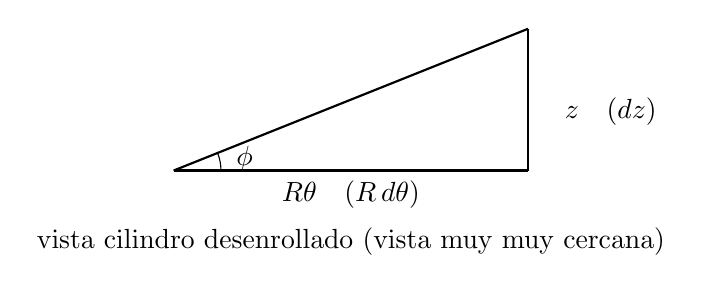
\begin{tikzpicture}[scale=1.5]
  \draw[thick] (0,0) -- (3,1.2); % hipotenusa
  \draw[thick] (0,0) -- (3,0);   % base
  \draw[thick] (3,0) -- (3,1.2); % lado
  \draw[dashed] (0,0) -- (0.8,0);
  \draw[dashed] (0,0) -- (0.8,0.32);
  \draw[-] (0.4,0) arc (0:21:0.4);
  \node at (0.6,0.1) {$\phi$};
  \node at (1.5,-0.6) {vista cilindro desenrollado (vista muy muy cercana)};
  \node at (3.7,0.5) {$z\quad(dz)$};
  \node at (1.5,-0.2) {$R\theta \quad(R\,d\theta)$};
\end{tikzpicture}
\end{center}
$$\tan\phi=\dfrac{z}{R\theta}=\dfrac{dz}{R\,d\theta}\quad\longrightarrow\quad z=R\theta\tan\phi$$

\textbf{Velocidad}\\
La velocidad es la derivada temporal de la posición desde un punto fijo.
% NOTA PARA REVISIÓN (agente B): el zip escribe der{(R e_r + R)}; por contexto debería ser R e_r + z e_z.
$$\marc{\vec{v}_P}{N}=\der{\vec{r}_{P}}{N}=\der{(R\vec{e}_r+R)}{N}{}= R\der{\vec{e}_r}{N}{}+R\dot\theta\tan\phi\,\vec{e}_z$$

\patotruco{No es necesario usar el teorema del transporte completo: usamos el trucazo (la demostración está en la Ayudantía 5). Como $\vec{e}_r$ y $\vec{e}_\theta$ giran solo en torno a $\vec{e}_z$, basta con $\dot{\vec{e}}_r=\dot\theta\vec{e}_\theta$ y $\dot{\vec{e}}_\theta=-\dot\theta\vec{e}_r$.}

Derivadas temporales de $\vec{e}_r$ y $\vec{e}_\theta$:
$$\transport{\vec{e}_r}{N}{A}=\dot\theta\vec{e}_z\times\vec{e}_r=\dot\theta\vec{e}_\theta$$
$$\transport{\vec{e}_\theta}{N}{A}=\dot\theta\vec{e}_z\times\vec{e}_\theta=-\dot\theta\vec{e}_r$$
y finalmente
$$\marc{\vec{v}_P}{N}=R\dot\theta\,\vec{e}_\theta+R\dot\theta\tan\phi\,\vec{e}_z$$

\textbf{Aceleración}\\
Al igual que antes, podemos simplemente derivar la velocidad:
$$\marc{\vec{a}_P}{N}=\der{\marc{\vec{v}_P}{N}{}}{N}{}=\der{\left(R\dot\theta\vec{e}_\theta+R\dot\theta\tan\phi\,\vec{e}_z\right)}{N}{}=(-R\dot\theta^2)\vec{e}_r+ R\ddot\theta\,\vec{e}_{\theta}+R\ddot\theta\tan\phi\,\vec{e}_z$$

\subsubsection*{Cinética}
\textbf{Diagrama de cuerpo libre}\\
Siempre se parte por un DCL, analizando las fuerzas que afectan a la masa. Recuerden que cada vez que eliminamos algo del DCL lo tenemos que reemplazar por una fuerza.
\begin{center}
\begin{tikzpicture}[>=Latex, scale=1.2]
    \shadedraw[ball color=gray!30] (0,0) circle (0.3) node {$m$};
    \draw[->, thick, azul] (0,0.3) -- (0,1.2) node[above] {$N_n$};
    \draw[->, thick, azul] (0.25,0.17) -- (1.2,0.75) node[above right] {$N_b$};
    \draw[->, thick, myred] (0,-0.3) -- (0,-1.2) node[below] {$mg$};
\end{tikzpicture}
\end{center}
Después del DCL se caracteriza cada fuerza vectorialmente:
$$\vec{F}_g=-mg\,\vec{e}_z$$
$$\vec{N}=N_b\vec{e}_b+N_n\vec{e}_n$$
En este caso no es necesario obtener las direcciones normal y binormal, porque más adelante se irán.

\textbf{Ecuación diferencial}\\
Ahora aplicamos el teorema de Trabajo y Energía. ¿Qué nos dice? (Discrepo con el nombre, porque en realidad es la derivada, pero cosas de la vida.) El teorema nos dice que la derivada (el cambio) de la energía cinética es igual a la potencia de las fuerzas.
$$\marc{P}{N}=\dfrac{d}{dt}(\marc{E_k}{N}{})$$
$$\marc{P}{N}=\marc{\vec{v}_P}{N}\cdot\sum \vec{F}$$
$$\marc{E_k}{N}=\dfrac{1}{2}m \marc{\vec{v}_P}{N}\cdot\marc{\vec{v}_P}{N}=\dfrac{1}{2}m \left(\marc{\vec{v}_P}{N}\right)^2$$
Reemplazando se tiene que
$$\marc{P}{N}=(-mg\vec{e}_z+N_b\vec{e}_b+N_n\vec{e}_n)\cdot\marc{\vec{v}_P}{N}\quad\longrightarrow\quad-mgR\dot\theta\tan\phi$$
% NOTA PARA REVISIÓN (agente B): en el zip la energía cinética se escribe con (R theta')tan^2(phi) en lugar de
% (R theta' tan(phi))^2; debería ser T = (1/2) m R^2 theta'^2 (1+tan^2 phi). Se deja tal cual.
$$\dfrac{d}{dt}(\marc{E_k}{N}{})=\dfrac{d}{dt}\left(\dfrac{1}{2}m((R\dot\theta)^2+(R\dot\theta)\tan^2\phi)\right)=mR\dot\theta (R\ddot\theta)(1+\tan^2\phi)$$
En la parte de las normales, se van; esto se puede ver claramente cuando expreso la velocidad como $\marc{v_P}{N}\vec{e}_t$ y hago el producto punto con la normal: da 0. Siguiendo con la igualdad se tiene que
$$mR\dot\theta (R\ddot\theta)(1+\tan^2\phi)=-mgR\dot\theta\tan\phi$$
$$m(R\ddot\theta)(1+\tan^2\phi)=-mg\tan\phi$$
\respuesta{$\displaystyle \ddot\theta=-\dfrac{g\tan\phi}{R(1+\tan^2\phi)}$}

\subsubsection*{Desplazamiento a máxima altura}
Se busca la máxima altura; para encontrarla tenemos que ver para qué valor de $\theta$ se consigue el máximo de $z=R\theta\tan\phi$. Podemos derivar e igualar a 0; de ahí se obtiene que en el punto de máxima altura $\dot\theta=0$. Con esta información podemos integrar el teorema de trabajo y energía (que ahora sí tiene sentido con el nombre; por eso, según yo, es el teorema integrado el que debería tener ese nombre).
$$\int_{0}^{t_f}\marc{P}{N}dt=\int_0^{t_f}\dfrac{d\left(E_k\right)}{dt}dt$$
$$\int_{0}^{t_f}-mgR\dot\theta\tan\phi\,dt=E_f-E_i$$
A mano izquierda hacemos un cambio de variable $\theta=f(t)$, mientras que al lado derecho tenemos la energía cinética final e inicial. Del análisis anterior sabemos que $\dot\theta=0$ en el punto que nos interesa (mayor altura), así que la energía cinética final es 0, y la inicial es, para $t=0$,
% NOTA PARA REVISIÓN (agente B): en el zip falta el factor 1/2 en E_i (debería ser (1/2) m R^2 theta'_0^2 (1+tan^2 phi)),
% lo que duplica theta_f - theta_0 y la componente z del desplazamiento. Se deja tal cual.
$$E_i=mR^2\dot\theta_0^2(1+\tan^2\phi)$$
$$\int_{0}^{t_f}-mgR\dot\theta\tan\phi\,dt\quad\dot\theta=\dfrac{d\theta}{dt}\quad\longrightarrow\quad\int_{\theta_0}^{\theta_f}-mgR\tan\phi\,d\theta=-mgR\tan\phi\,(\theta_f-\theta_0)$$
$$-mR^2\dot\theta_0^2(1+\tan^2\phi)=-mgR\tan\phi\,(\theta_f-\theta_0)$$
$$\theta_f = \theta_0 +\frac{R\,\dot{\theta}_0^2\,\bigl(1 + \tan^2\phi\bigr)}{g\,\tan\phi}$$
Con esto basta con evaluarlo en el desplazamiento de una partícula, que se define de manera más profesional como
$$\int_{t_i}^{t_f}\marc{\vec{v}}{N}dt$$
pero como la velocidad es la derivada de la posición, basta con evaluar en los extremos de la función posición:
\respuesta{$\displaystyle \vec{r}_{t_f}-\vec{r}_{t_i}=R\left(\cos\theta_f-\cos\theta_0\right)\vec{e}_x+R\left(\sin\theta_f-\sin\theta_0\right)\vec{e}_y+\frac{R^2\,\dot{\theta}_0^2\,\bigl(1 + \tan^2\phi\bigr)}{g}\vec{e}_z$}

\end{solucion}

% =========================================================================
% Capítulo 2: Cinética de la partícula
% Tema 01: Dinámica de la partícula
% Problema 18: Partícula con resorte en brazo giratorio
% =========================================================================
\subsubsection{Partícula con resorte en brazo giratorio}

Una partícula de masa $m$ está unida a un resorte lineal con constante elástica $K$ y longitud natural $r_0$. El otro extremo del resorte está conectado, en el punto $P$, al extremo libre de un brazo rígido sin masa de longitud $l$. El brazo está articulado en su otro extremo $O$ y gira en una trayectoria circular con una rapidez angular constante $\omega$. Sabiendo que la gravedad actúa hacia abajo y definiendo $r$ como la longitud del resorte y $\theta$ como el ángulo de la partícula respecto a la vertical, realice lo siguiente:

\begin{enumerate}
    \item Defina los marcos de referencia y sistemas de coordenadas adecuados.
    \item Analice la cinemática de la partícula determinando sus vectores de posición y velocidad en función de las coordenadas generalizadas.
    \item Analice la cinética del sistema para determinar las ecuaciones diferenciales del movimiento.
\end{enumerate}

\begin{figure}[!ht]
    \centering
    \begin{tikzpicture}[>=Latex, scale=1.5]
        % --- Parámetros ---
        \def\ang{-40}      % Ángulo de inclinación (omega*t y theta coinciden en el dibujo)
        \def\Lbar{2.0}     % Longitud del brazo l
        \def\Lspring{1.5}  % Longitud del resorte r

        % Coordenadas
        \coordinate (O) at (0,0);
        \coordinate (P) at (\ang:\Lbar);
        \coordinate (M) at (\ang+15:{\Lbar+\Lspring});

        % --- 1. Soporte y Pivote ---
        \fill[pattern=north east lines] (-0.5, 0) rectangle (0.5, 0.2);
        \draw[thick] (-0.5, 0) -- (0.5, 0);
        \filldraw[gray] (O) circle (2pt);
        \node[below left, xshift=-3pt] at (O) {$O$};

        % --- 2. Brazo Giratorio ---
        \draw[line width=3.5pt, black,line cap=round] (O) -- (P);
        \draw[line width=3pt, gray!40,line cap=round] (O) -- (P);
        \draw[thick,line cap=round ] (O) -- (P) node[midway, above right] {$l$};
        \filldraw (P) circle (0.5pt) node[below left, yshift=5pt] {$P$};
        \filldraw (O) circle (0.5pt);

        % --- 3. Resorte y Masa ---
        \draw[decoration={coil, aspect=0.4, segment length=3pt, amplitude=3pt, pre length=3pt, post length=3pt}, decorate, thick] (P) -- (M);
        \node at ($(P)!0.5!(M)$) [below left=2pt] {$K$};
        
        \shadedraw[ball color=white] (M) circle (3.5pt) node[] {$m$};

        % --- 4. Cotas y Referencias ---
        % Referencia Vertical
        \draw[dashed, gray] (O) -- (0, -2.0);
        \draw[dashed, gray] (P) -- ++ (0, -2.0);
        
        % Ángulo omega*t (Referido al brazo)
        \draw[->, thick] (0, -0.8) arc (-90:\ang:0.8);
        \node at ({(\ang-90)/2}:1.1) {$\omega t$};

        % Ángulo theta (Referido a la masa - dibujado un poco más abajo)
        \draw[->, thick] (P)++(0,-1.6) arc (-90:\ang+30:1.6) node[midway, above] {$\theta$};

        % Cota r (Longitud del resorte)
        % Calculamos puntos desplazados para la cota paralela
        \draw[thin, |<->|] ($(P)+(\ang+90:0.4)$) -- ($(M)+(\ang+90:0.4)$) node[midway, above right] {$r$};

    \end{tikzpicture}
    \caption{Sistema de partícula unida a un resorte acoplado a un brazo en rotación forzada.}
    \label{fig:resorte_brazo_giratorio}
\end{figure}
\subsubsection{Desplazamiento virtual en péndulo sobre columna rotatoria}

Una masa $m$ (punto $P$) está suspendida mediante una varilla rígida de longitud $L_2$ desde el extremo de un brazo horizontal de longitud $L_1$. El brazo está unido rígidamente a una columna vertical que rota con una velocidad angular $\dot{\phi}$ alrededor del eje $Z$. El péndulo oscila en el plano vertical generado por la columna y el brazo, definido por el ángulo $\theta$ con la vertical. Considerando que la gravedad actúa hacia abajo, realice lo siguiente:

\begin{enumerate}
    \item Defina los vectores de posición del punto $P$ en un sistema de coordenadas inercial.
    \item Determine el vector de velocidad del punto $P$.
    \item Determine la expresión para el \textbf{desplazamiento virtual} $\delta \vec{r}_P$ del punto $P$ en términos de las coordenadas generalizadas y sus variaciones.
\end{enumerate}

\begin{figure}[htbp]
    \centering
    \begin{tikzpicture}[>=Latex, scale=1.4]
        % --- Parámetros ---
        \def\ColW{0.8}    % Ancho columna
        \def\ColH{3.5}    % Alto columna
        \def\Lone{2.8}    % Longitud L1
        \def\Ltwo{2.2}    % Longitud L2
        \def\angTheta{25} % Ángulo theta
        
        % Coordenadas
        \coordinate (Base) at (0,0);
        \coordinate (Top) at (0, \ColH);
        \coordinate (ArmStart) at (0, \ColH-0.5);
        \coordinate (ArmEnd) at (\Lone, \ColH-0.5);
        \coordinate (Mass) at ($(ArmEnd) + ({sin(\angTheta)*\Ltwo}, {-cos(\angTheta)*\Ltwo})$);

        % --- 1. Base y Columna ---
        % Base soporte
        \fill[pattern=north east lines] (-0.8, -0.2) rectangle (0.8, 0);
        \draw[thick] (-0.8, 0) -- (0.8, 0);
        %\draw[fill=gray!20] (0,0.1) ellipse (0.9 and 0.15); % Base de la columna visual

        % Columna (Cilindro)
        \fill[left color=gray!30, right color=gray!10, middle color=gray!5] (-\ColW/2,0) rectangle (\ColW/2, \ColH);
        \draw[thick] (-\ColW/2, 0) rectangle (\ColW/2, \ColH);
        
        % Tapa columna (Elipse superior)
        %\draw[fill=gray!20] (0, \ColH) ellipse (\ColW/2 and 0.15);
        
        % Eje Z
        \draw[->, thick] (0, \ColH) -- (0, \ColH+1.0) node[right] {$Z$};

        % --- 2. Brazo L1 ---
        \draw[line width=4pt, gray!40] (0, \ColH-0.6) -- (0, \ColH-0.4) -- (\Lone, \ColH-0.4) -- (\Lone, \ColH-0.6) -- cycle;
        \draw[thick] (0, \ColH-0.6) -- (\Lone, \ColH-0.6);
        \draw[thick] (0, \ColH-0.4) -- (\Lone, \ColH-0.4);
        \draw[thick] (\Lone, \ColH-0.6) -- (\Lone, \ColH-0.4);
        
        % Cota L1
        \draw[|<->|] (0, \ColH-0.2) -- (\Lone, \ColH-0.2) node[midway, above] {$L_1$};

        % --- 3. Péndulo L2 y Masa ---
        \draw[thick] (ArmEnd) -- (Mass) node[midway, right] {$L_2$};
        
        % Masa P
        \shadedraw[ball color=gray!30!white] (Mass) circle (0.25) node[] (Mass) {$m$};
        \node[left, xshift=-8pt] at (Mass) {$P$};

        % --- 4. Ángulos y Rotación ---
        % Referencia Vertical en extremo del brazo
        \draw[dashed] (ArmEnd) -- ($(ArmEnd) + (0, -2.0)$);
        
        % Ángulo Theta
        \draw[->] ($(ArmEnd) + (0, -1.2)$) arc (270:{270+\angTheta}:1.2);
        \node at ($(ArmEnd) + ({sin(\angTheta/2)*0.9}, {-cos(\angTheta/2)*0.9})$) [] {$\theta$};

        % Rotación Phi
        \draw[->, thick] (-0.8, 1.5) arc (180:360:0.8 and 0.3);
        \node[right] at (0.8, 1.5) {$\dot{\phi}$};

        % --- 5. Gravedad ---
        \draw[->, thick] (2.5, 2.5) -- (2.5, 1.5) node[midway, right] {$g$};

    \end{tikzpicture}
    \caption{Sistema de péndulo suspendido de un brazo en rotación acimutal.}
    \label{fig:pendulo_rotatorio}
\end{figure}

\newpage
\subsection{Solución Modelo}

El siguiente ejemplo ilustra la metodología general de resolución (marcos de
referencia, diagrama de cuerpo libre y segunda ley de Newton). No corresponde
a la solución de un problema numerado específico, sino a un esquema de
referencia para resolver los problemas anteriores.

\begin{sol}[{Solución ejemplo}]
Para los problemas siempre partimos definiendo los marcos de referencia y los sistemas de coordenadas a usar, también es de utilidad tener en cuenta la transformación de un sistema a otro sistema.
\begin{marcos}
A continuación presentare los marcos de referencia (a los objetos que están asociados) y los sistemas de coordenadas asociados a ellos
    \begin{itemize}
    \item $\mathcal{N}$ Inercial (Suelo) $\longrightarrow\{\vec{E}_x;\vec{E}_y;\vec{E}_z\}$
    \item $\mathcal{D}$ Gira con el disco $\longrightarrow\{\vec{e}_x;\vec{e}_y;\vec{e}_z\}$
    \item $\mathcal{A}$ Gira con el disco $\longrightarrow\{\vec{e}_r;\vec{e}_\phi;\vec{e}_\theta\}$
    \item $\mathcal{B}$ Gira con el disco $\longrightarrow\{\vec{u}_x;\vec{u}_y;\vec{u}_z\}$
    \item $\mathcal{C}$ Gira con el disco $\longrightarrow\{\vec{e}_r;\vec{e}_\theta;\vec{e}_z\}$
\end{itemize}
\begin{center}
    % Primera minipage (lado izquierdo)
    \begin{minipage}{0.48\textwidth}
        \centering
        \begin{tikzpicture}[scale=1.2] % Ajusta el escala si es necesario
            \Polaresxyz{\theta}{E}{e}{blue}{green!60!black}
        \end{tikzpicture}
    \end{minipage}
    \hfill % Esto añade espacio elástico entre las dos imágenes
    % Segunda minipage (lado derecho)
    \begin{minipage}{0.48\textwidth}
        \centering
        \begin{tikzpicture}[scale=1.2]
            \Polaresrtz{\phi}{E}{e}{red}{orange} % Ejemplo con otros valores
        \end{tikzpicture}
    \end{minipage}
\end{center}
$$\vec{e}_x=\cos{(\theta)}\vec{E}_x+\sin{(\theta)}\vec{E}_y$$
$$\vec{e}_y=-\sin{(\theta)}\vec{E}_x+\cos{(\theta)}\vec{E}_y$$
$$\vec{e}_z=\vec{E}_z$$
\end{marcos}

\begin{cinematicaUnificada}{Análisis Cinemático del Punto P}
        El análisis cinemático, tiene en consideración el movimiento de la partícula, solo el movimiento no las causas, ni nada externo por ende primero tenemos que definir los vectores que nos ayudaran a analizar.

        
        \subtitulo{Posición y Velocidades Angulares}
        Siempre que nosotros queremos definir la posición lo que nos importa es que sepamos que el punto del cual la definimos es un punto el cual no se mueve, osea velocidad $\vec{0}$, dado que asi no nos generara problemas en un futuro
        \begin{equation}
            \vec{r}_P=
        \end{equation}
        Y para el caso de las velocidades angulares de los marcos de referencia se pueden obtener mediante la regla de la mano derecha y ver en que dirección gira. Con esto se llega a lo siguiente
        \begin{itemize}
            \item $\velang{N}{A}=\Omega\vec{e}_z$
        \end{itemize}

        \subtitulo{Velocidad} % <--- Aquí creamos la separación interna
        Siempre que nosotros queremos calcular la velocidad inercial de una partícula tenemos que derivar respecto a un observador en el marco de referencia inercial, un vector el cual sea respecto a un punto inercial.
        \begin{equation}
            \marc{}{N}\vec{v}_P=\der{}{N}\vec{r}_p=\der{}{N}\left(\right)
        \end{equation}
        Mediante el uso del teorema del trasporte podemos resolver y llega a 
        \begin{equation}
            \marc{}{N}\vec{v}_P=\transportad{\vec{r}_P}{N}{A}
        \end{equation}
        
        
        
        \begin{equation}
            \marc{}{N}\vec{v}_P=\transD{r\vec{e}_r}{\Omega\vec{e}_z}{N}{A}{\vec{t}_p}
        \end{equation}
        Desarrollando el teorema del transporte el termino 1
        \begin{align}
            \der{}{A}\left(r\vec{e}_r\right)=
        \end{align}
        Por otro lado el segundo termino del teorema del transporte
        \begin{align}
            \Omega\vec{e}_z\times r\vec{e}_r=
        \end{align}

        \subtitulo{Aceleración} % <--- Otra separación interna
        Para calcular la aceleración basta simplemente con repetir el proceso y derivar la velocidad previamente calculada, respecto al marco de referencia inercial $\mathcal{N}$
        \begin{equation}
            \marc{}{N}\vec{a}_P=\der{}{N}\marc{}{N}\vec{v}_p=\der{}{N}\left(\right)
        \end{equation}
        Mediante el uso del teorema del trasporte podemos resolver y llega a 
        \begin{equation}
            \marc{}{N}\vec{a}_P=\transportad{\marc{}{N}\vec{v}_p}{N}{A}
        \end{equation}
        
        
        
        \begin{equation}
            \marc{}{N}\vec{a}_P=\transD{r\vec{e}_r}{\Omega\vec{e}_z}{N}{A}{\marc{}{N}\vec{v}_p}
        \end{equation}
        Desarrollando el teorema del transporte el termino 1
        \begin{align}
            \der{}{A}\left(r\vec{e}_r\right)=
        \end{align}
        Por otro lado el segundo termino del teorema del transporte
        \begin{align}
            \Omega\vec{e}_z\times r\vec{e}_r=
        \end{align}

    \end{cinematicaUnificada}

\end{sol}
